\documentclass[11pt]{article} \usepackage{fullpage} \usepackage{graphicx} \usepackage{epstopdf} \usepackage{color} \usepackage{psfrag} \usepackage{pdfsync}\usepackage{indentfirst}\usepackage{subfigure}\usepackage{float}\usepackage[section]{placeins}
\usepackage{enumerate}
\usepackage{multirow}
\usepackage{amsfonts, fullpage, graphics} 
\usepackage{algorithm,algorithmic}
\usepackage{amsmath,amssymb,amsthm,bm,hyperref}
\usepackage{dsfont}
\usepackage[parfill]{parskip}
\usepackage[margin=1in]{geometry}
\newcommand{\Lagr}{\mathcal{L}}
\newcommand{\norm}[1]{\left\lVert#1\right\rVert}
\newcommand{\floor}[1]{\lfloor #1 \rfloor}
\newcommand{\todo}[1]{}
\renewcommand{\todo}[1]{{\color{red} TODO: {#1}}}
\newcommand\independent{\protect\mathpalette{\protect\independenT}{\perp}}
\newcommand{\obar}[1]{\mkern 1.5mu\overline{\mkern-1.5mu#1\mkern-1.5mu}\mkern 1.5mu}
\def\independenT#1#2{\mathrel{\rlap{$#1#2$}\mkern2mu{#1#2}}}
\newcommand{\rpm}{\sbox0{$1$}\sbox2{$\scriptstyle\pm$}
  \raise\dimexpr(\ht0-\ht2)/2\relax\box2 }
\usepackage{xspace}
\newcommand{\latex}{\LaTeX\xspace}
\setlength{\parindent}{2em}

\usepackage{listings}
\usepackage{color} %red, green, blue, yellow, cyan, magenta, black, white
\definecolor{mygreen}{RGB}{28,172,0} % color values Red, Green, Blue
\definecolor{mylilas}{RGB}{170,55,241}
\DeclareMathOperator{\E}{\mathbb{E}}
\DeclareMathOperator*{\argmax}{arg\,max}
\DeclareMathOperator*{\argmin}{arg\,min}

\begin{document}

{\parindent 0pt \begin{tabular}[t]{l} 16-720 Computer Vision \\ Spring 2020 \end{tabular}}%  \hfill XX/XX/14 \vskip 0.2in }
\parindent 0pt \parskip 8pt
\begin{center} \large\bf Homework 4 \end{center}
\begin{center} \large\bf Zongwen Mu, Andrew ID: zongwenm \end{center}
\bigskip


\section{Theory}

\setlength{\parindent}{2em}  

\paragraph{Q1.1}~{}

For given point $\bold{x}$, we have $\tilde{x_1} = \tilde{x_2} = \begin{bmatrix} 0 & 0 & 1 \end{bmatrix}^\mathbf{T}$. Therefore, we have:
\begin{align}
	\tilde{x_2}^\mathbf{T}F\tilde{x_1} & = 0 \\
	\begin{bmatrix}
	0 & 0 & 1
	\end{bmatrix}
	\begin{bmatrix}
	F_{11} & F_{12} & F_{13} \\
	F_{21} & F_{22} & F_{23} \\
	F_{31} & F_{32} & F_{33}
	\end{bmatrix}
	\begin{bmatrix}
	0 \\ 0 \\ 1
	\end{bmatrix}
	& = 0 \\
	F_{33} & = 0 
\end{align}

\paragraph{Q1.2}~{}

For pure translation parallel to x-axis:
\begin{align}
	t & = \begin{bmatrix} t_1 \\ 0 \\ 0 \end{bmatrix} \\
	R & = \begin{bmatrix} 1 & 0 & 0 \\ 0 & 1 & 0 \\ 0 & 0 & 1 \end{bmatrix} \\
	E & = tR \\
	& = \begin{bmatrix}
	0 & 0 &0 \\
	0 & 0 & -t_1 \\
	0 & t_1 & 0
	\end{bmatrix}
\end{align}

Suppose that $\tilde{x_1}^T = \begin{bmatrix} a_1 & a_2 & 1\end{bmatrix}$ and $\tilde{x_2}^T = \begin{bmatrix} b_1 & b_2 & 1\end{bmatrix}$, we have:
\begin{align}
	l_{1}^T & = \tilde{x_2}^TE \\
	& = \begin{bmatrix} b_1 & b_2 & 1\end{bmatrix}\begin{bmatrix}
	0 & 0 &0 \\
	0 & 0 & -t_1 \\
	0 & t_1 & 0
	\end{bmatrix} \\
	& = \begin{bmatrix} 0 & t_1 & -b_2t_1 \end{bmatrix} \\
	l_{2}^T & = \tilde{x_1}^TE^T \\
	& = \begin{bmatrix} a_1 & a_2 & 1\end{bmatrix}\begin{bmatrix}
	0 & 0 &0 \\
	0 & 0 & t_1 \\
	0 & -t_1 & 0
	\end{bmatrix} \\
	& = \begin{bmatrix} 0 & -t_1 & a_2t_1 \end{bmatrix}
\end{align}

Thus, we could acquire epipolar lines in the two cameras: $t_1y_1 - b_2t_1 = 0, -t_1y_2 + a_2t_1 = 0$. Both do not contain $x$ component, so they are parallel to the x-axis.

\paragraph{Q1.3}~{}

Assume that the coordinate of the object in 3D world is $\begin{bmatrix} u & v & w\end{bmatrix}^T$, and let $\begin{bmatrix} x_i & y_i \end{bmatrix}^T$ be the position at time $i$. Thus we have:
\begin{align}
	\begin{bmatrix} x_1 \\ y_1 \\ 1 \end{bmatrix} & = K\left(R_1\begin{bmatrix}u \\ v \\ w\end{bmatrix} + t_1\right) \\
	\begin{bmatrix} u \\ v \\ w \end{bmatrix} & = R_1^{-1}\left(K^{-1}\begin{bmatrix}x_1 \\ y_1 \\ 1\end{bmatrix} - t_1\right) \\
	& = R_1^{T}K^{-1}\begin{bmatrix}x_1 \\ y_1 \\ 1\end{bmatrix} - R_1^{T}t_1 \\
	\begin{bmatrix} x_2 \\ y_2 \\ 1 \end{bmatrix} & = K\left(R_2\begin{bmatrix}u \\ v \\ w\end{bmatrix} + t_2\right) \\
	& = K\left(R_2\left(R_1^{T}K^{-1}\begin{bmatrix}x_1 \\ y_1 \\ 1\end{bmatrix} - R_1^{T}t_1\right) + t_2\right) \\
	& = KR_2R_1^{T}K^{-1}\begin{bmatrix}x_1 \\ y_1 \\ 1\end{bmatrix} - KR_2R_1^{T}t_1 + Kt_2
\end{align}

Therefore:
\begin{align}
	R_{rel} & = KR_2R_1^TK^{-1} \\
	t_{rel} & = -KR_2R_1^Tt_1 + Kt_2 \\
	E & = t_{rel} \times R_{rel} \\
	F & = \left(K^{-1}\right)^TEK^{-1} \\
	& = \left(K^{-1}\right)^T\left(t_{rel} \times R_{rel}\right)K^{-1}
\end{align}

\paragraph{Q1.4}~{}

Assume that the distance between object and mirror is $d$, thus the distance between two images is $2d$ and there is pure translation:
\begin{align}
	R_{rel} & = \mathbf{I} \\
	t_{rel} & = \begin{bmatrix} t_x & t_y & t_z \end{bmatrix} \\
	F & = \left(K^{-1}\right)^T\left(t_{rel} \times R_{rel}\right)K^{-1} \\
	& = \left(K^{-1}\right)^T \begin{bmatrix} 0 & t_z & -t_y \\ -t_z & 0 & t_x \\ t_y & -t_x & 0 \end{bmatrix}K^{-1}
\end{align} 
Thus, fundamental matrix $\bold{F}$ is a skew-symmetric matrix.

\section{Fundamental Matrix Estimation}

\paragraph{Q2.1}~{}

The recovered matrix $\bold{F}$ is:
\begin{equation}
	\bold{F} = \begin{bmatrix}
	9.78833286e-10 & -1.32135929e-07 & 1.12585666e-03 \\
	-5.73843315e-08 & 2.96800276e-09 & -1.17611996e-05 \\
	-1.08269003e-03 & 3.04846703e-05 & -4.47032655e-03
	\end{bmatrix}
\end{equation}
and example output image is shown below:
\begin{figure}[H]
\centering
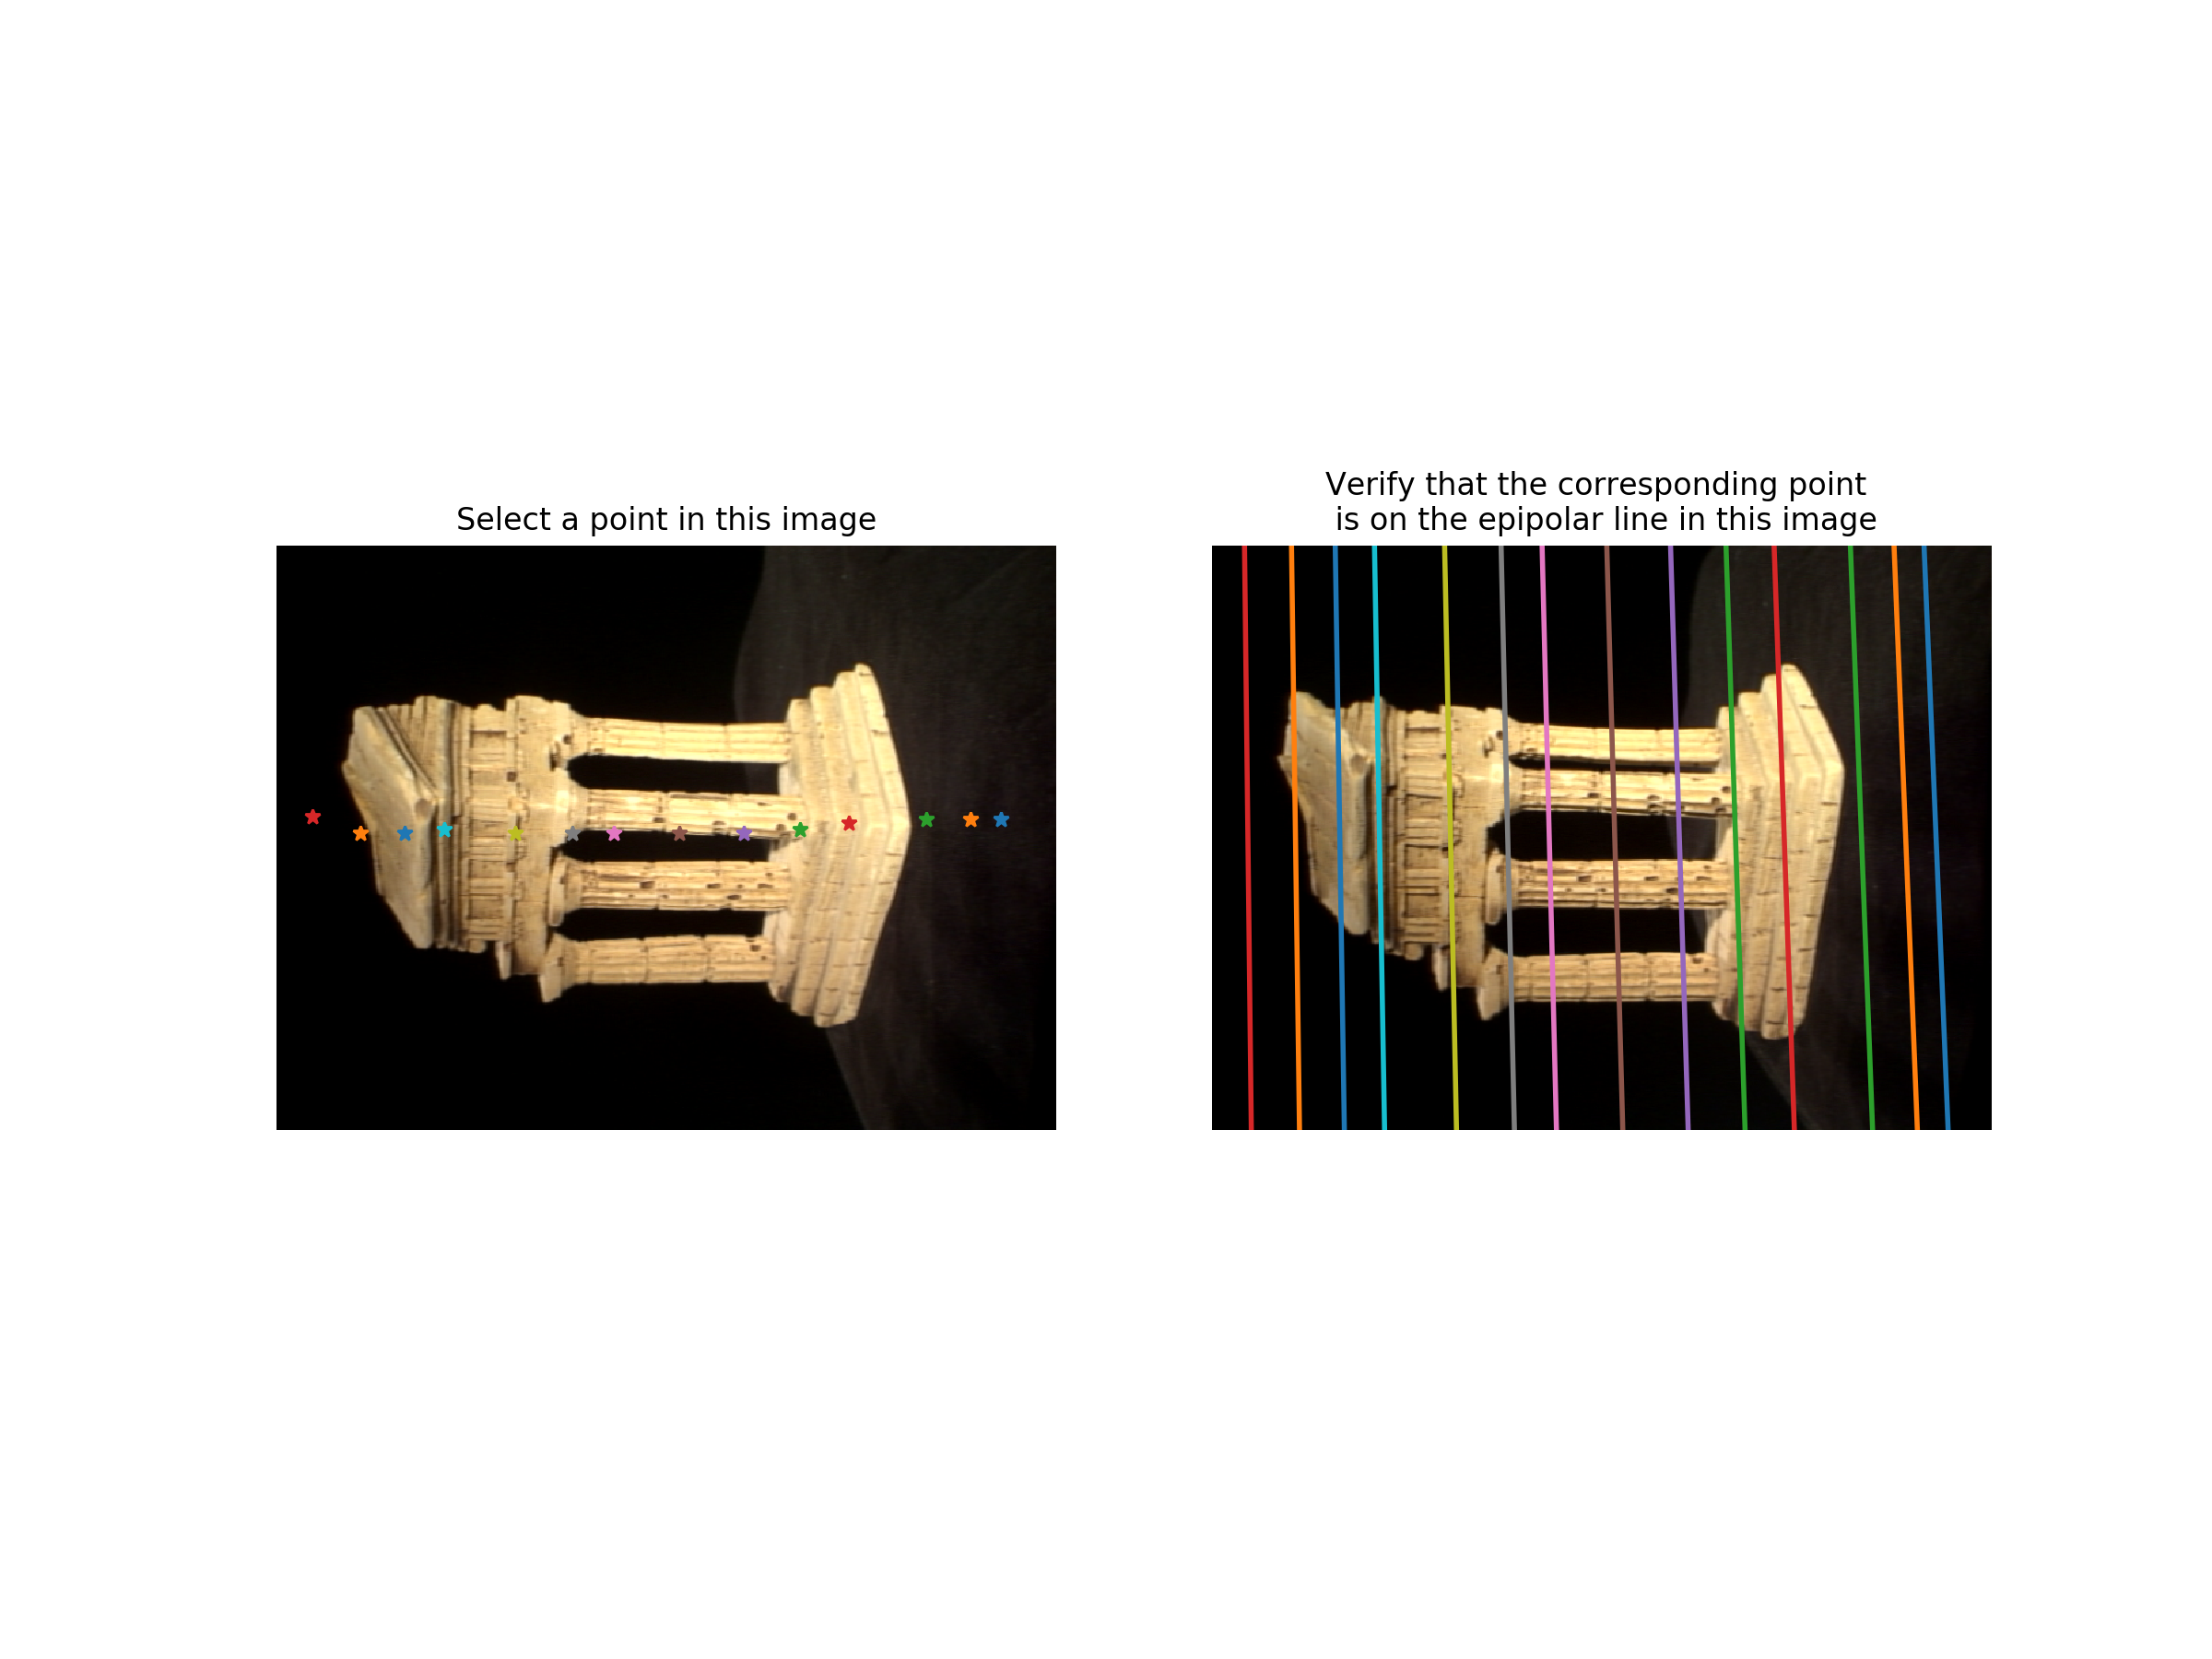
\includegraphics[width=0.9\textwidth]{results/q2_1.png}
\caption{Visualized Epipolar Lines}
\end{figure}

\section{Metric Reconstruction}

\paragraph{Q3.1}~{}

$\bold{E}$ can be calculated by $\bold{K_2^TFK_1}$. Using the eight-point algorithm, the estimated $\bold{E}$ is:
\begin{equation}
	\bold{E} = \begin{bmatrix}
	2.26268684e-03 & -3.06552495e-01 & 1.66260633e+00 \\
	-1.33130407e-01 & 6.91061098e-03 & -4.33003420e-02 \\
	-1.66721070e+00 & -1.33210351e-02 & -6.72186431e-04
	\end{bmatrix}
\end{equation}

\paragraph{Q3.2}~{}

Suppose $\bold{C}_{1i}$ and $\bold{C}_{2i}$ is the $i$th row for $\bold{C}_1$ and $\bold{C}_2$. If $\tilde{\bold{w}_i}$ is a $4 \times 1$ vector of the 3D coordinate in the homogeneous form, we have:
\begin{align}
	\bold{C}_1\bold{\tilde{w}}_i & = \widehat{\bold{x}_{1i}} \\
	\begin{bmatrix} \bold{C}_{11} \\ \bold{C}_{12} \\ \bold{C}_{13} \end{bmatrix}\begin{bmatrix} u_{i} \\ v_{i} \\ w_{i} \\ 1 \end{bmatrix} & = \begin{bmatrix} x_{1i} \\ y_{1i} \\ 1 \end{bmatrix} \\
	\bold{C}_2\bold{\tilde{w}}_i & = \widehat{\bold{x}_{2i}} \\
	\begin{bmatrix} \bold{C}_{21} \\ \bold{C}_{22} \\ \bold{C}_{23} \end{bmatrix}\begin{bmatrix} u_{i} \\ v_{i} \\ w_{i} \\ 1 \end{bmatrix} & = \begin{bmatrix} x_{2i} \\ y_{2i} \\ 1 \end{bmatrix}
\end{align}

Therefore, we have:
\begin{equation}
	\bold{A}_i = \begin{bmatrix} x_{1i}\bold{C}_{13} - \bold{C}_{11} \\ y_{1i}\bold{C}_{13} - \bold{C}_{12} \\ x_{2i}\bold{C}_{23} - \bold{C}_{21} \\ y_{2i}\bold{C}_{23} - \bold{C}_{22} \end{bmatrix}
\end{equation}

\section{3D Visualization}

\paragraph{Q4.1}~{}

Choose window size $20$, the matched result is shown below:
\begin{figure}[H]
\centering
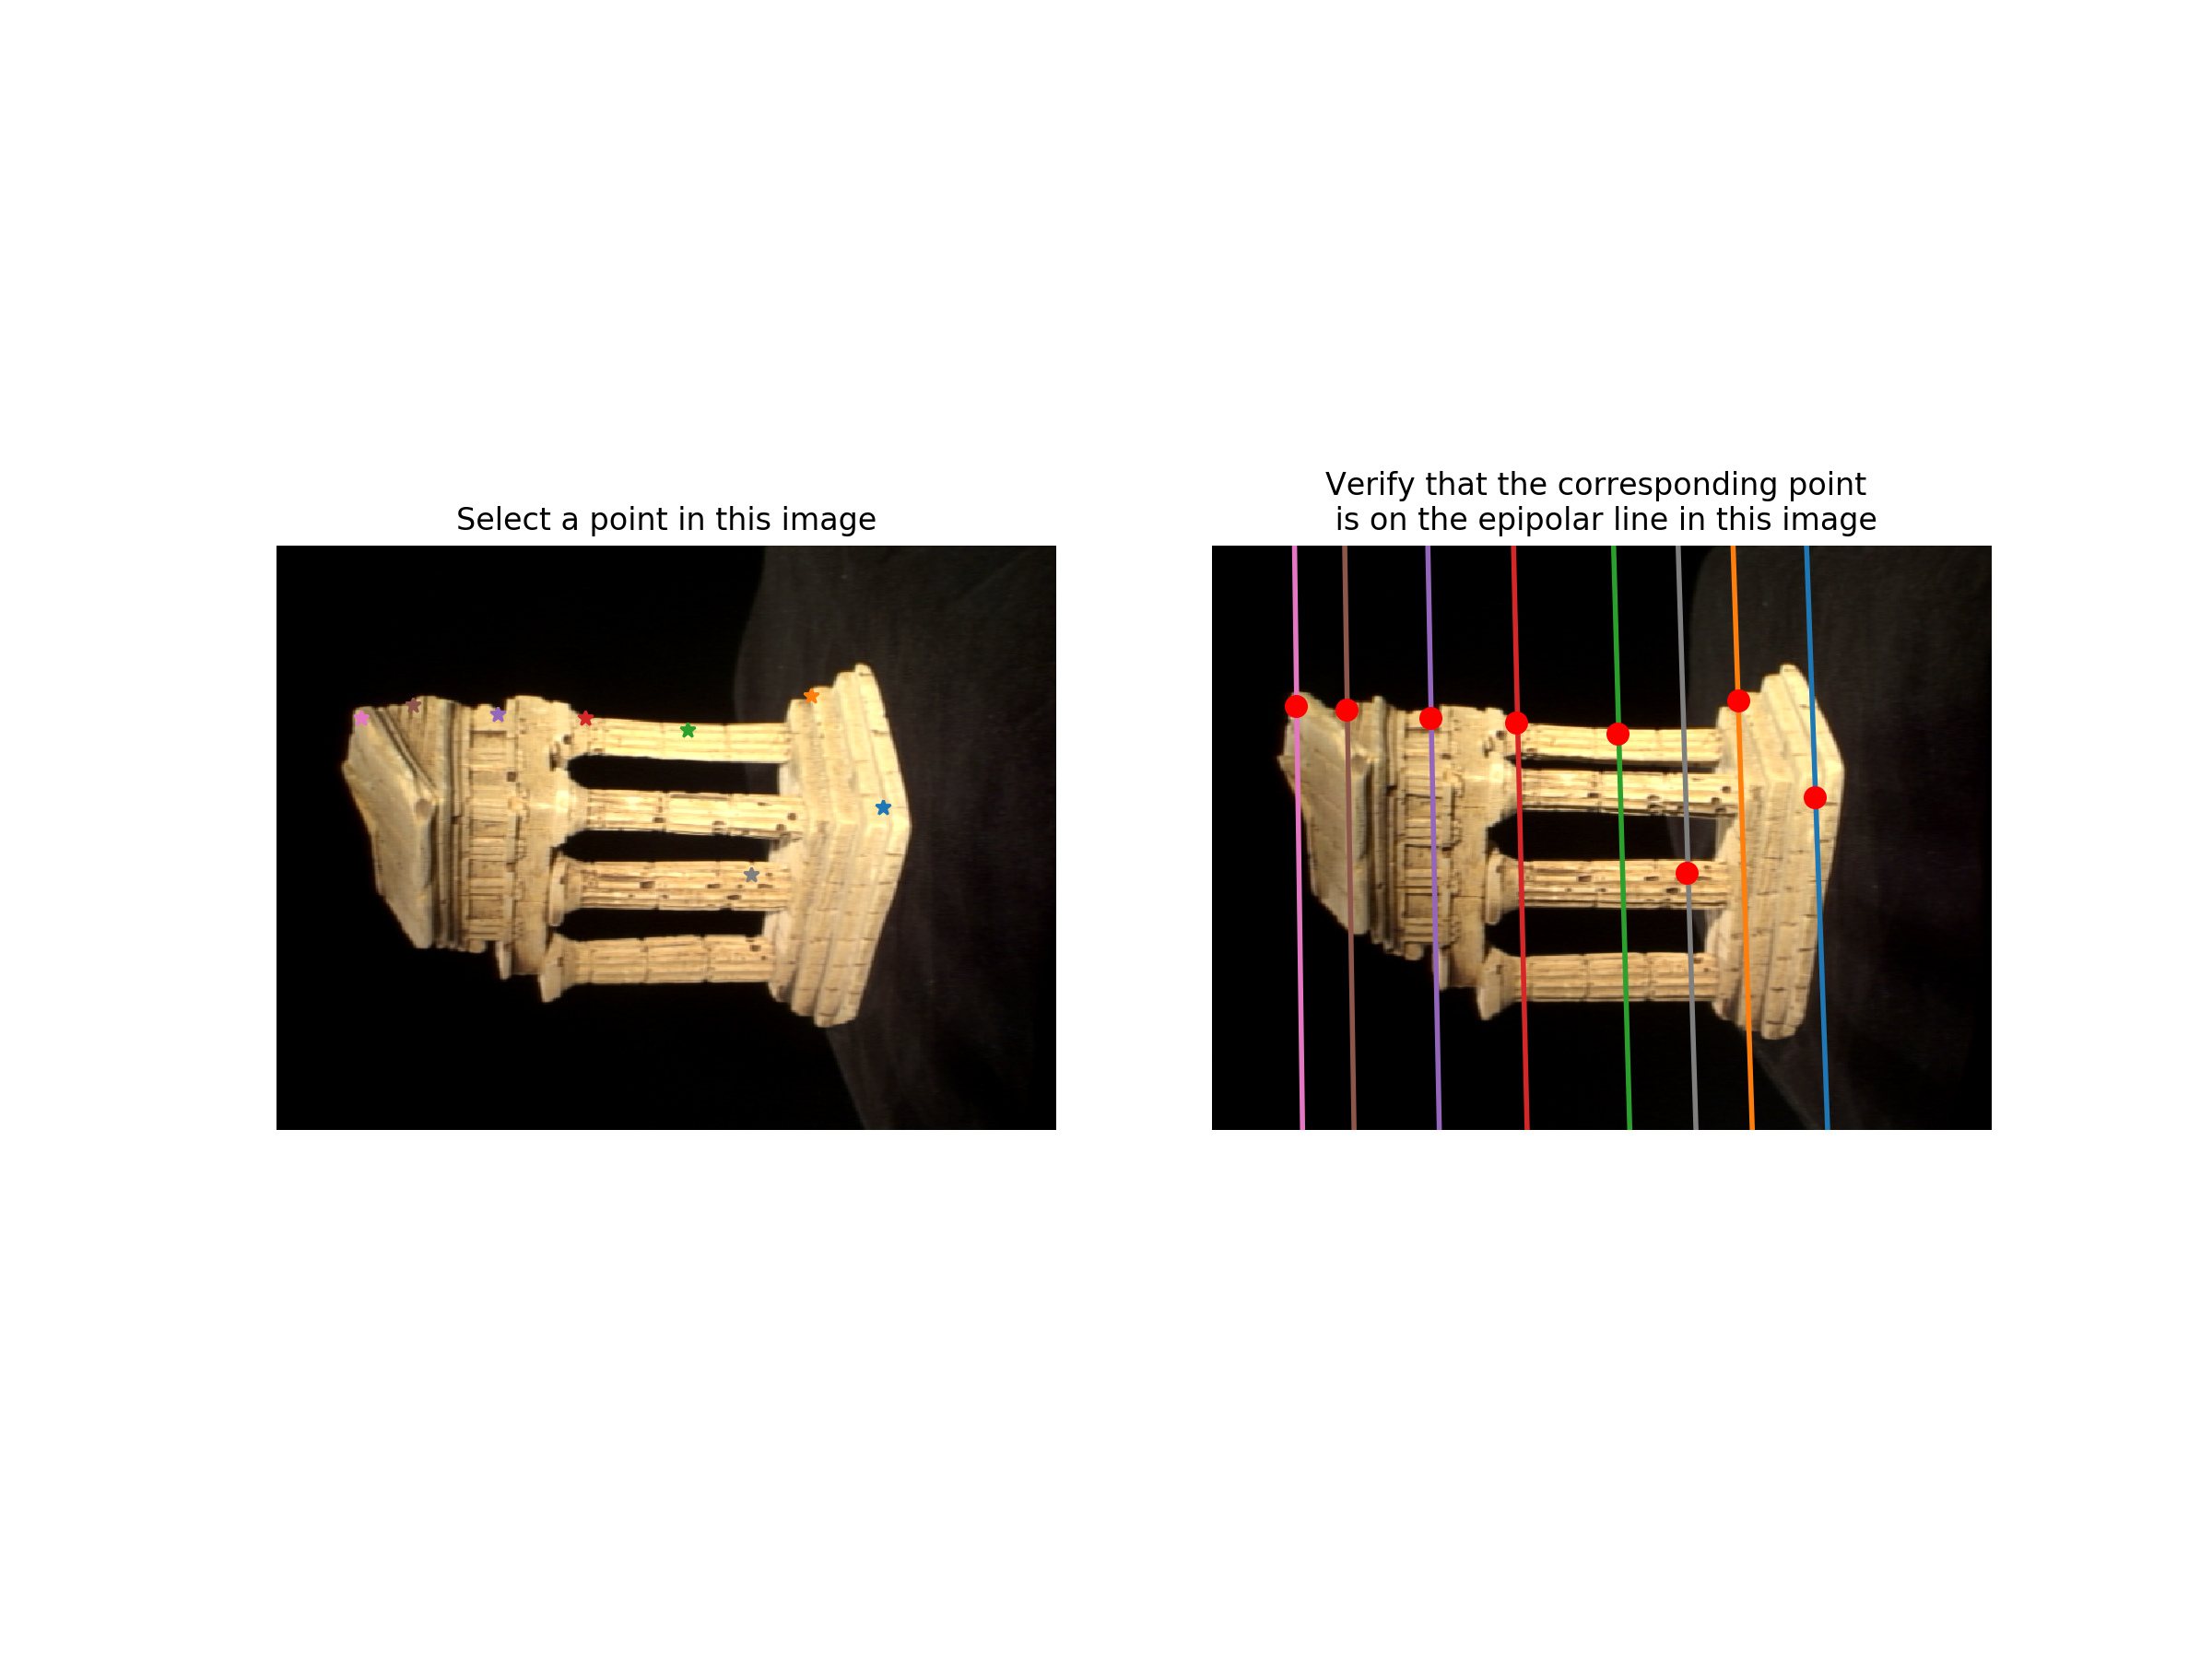
\includegraphics[width=0.7\textwidth]{results/q4_1.png}
\caption{Corresponding Points}
\end{figure}

\paragraph{Q4.2}~{}
The results for $3D$ visualization is shown below:
\begin{figure}[H]
\centering
\subfigure[]{
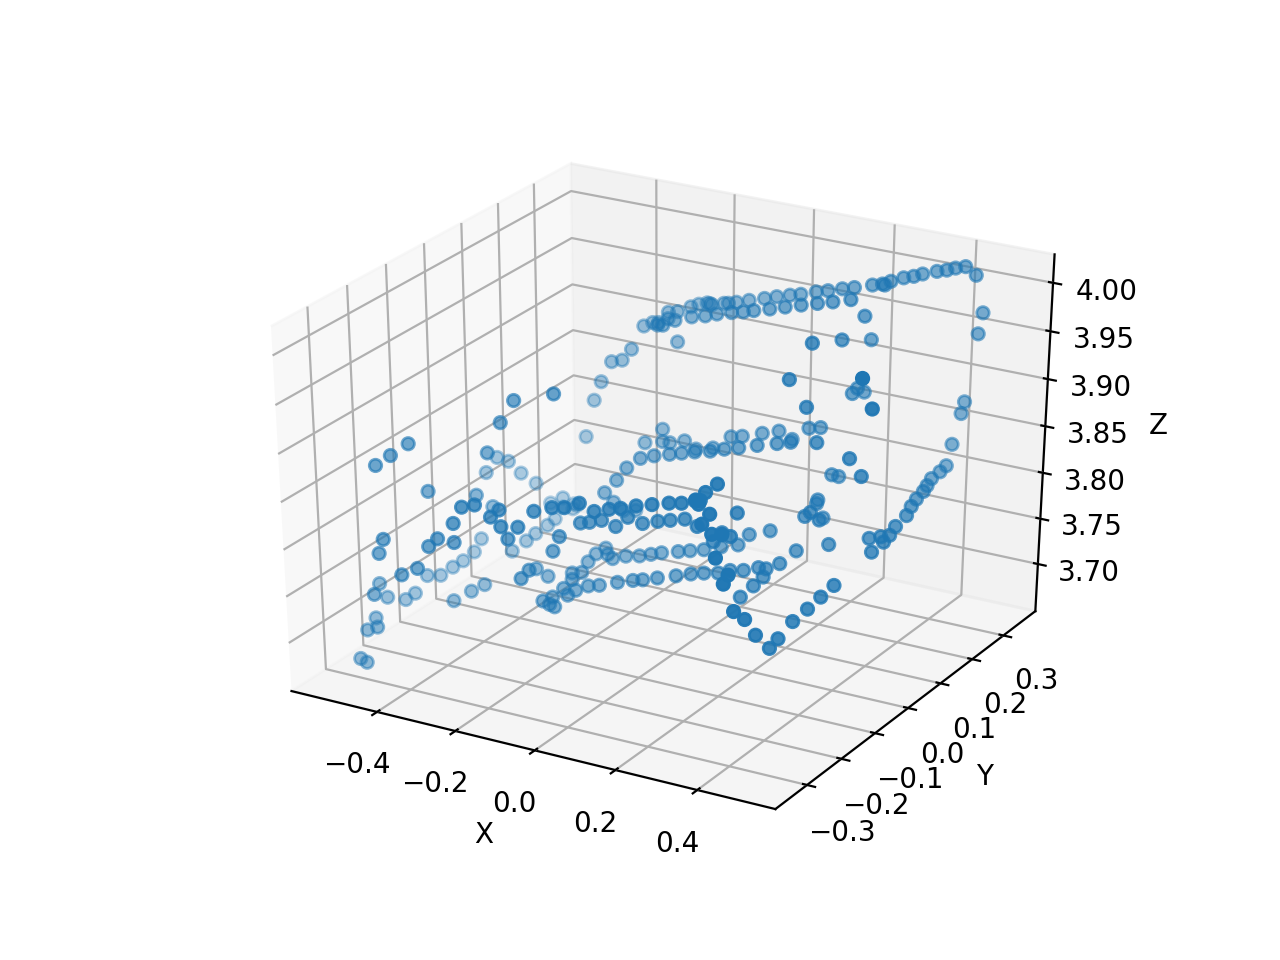
\includegraphics[width=0.4\textwidth]{results/q4_2_1.png}}
\subfigure[]{
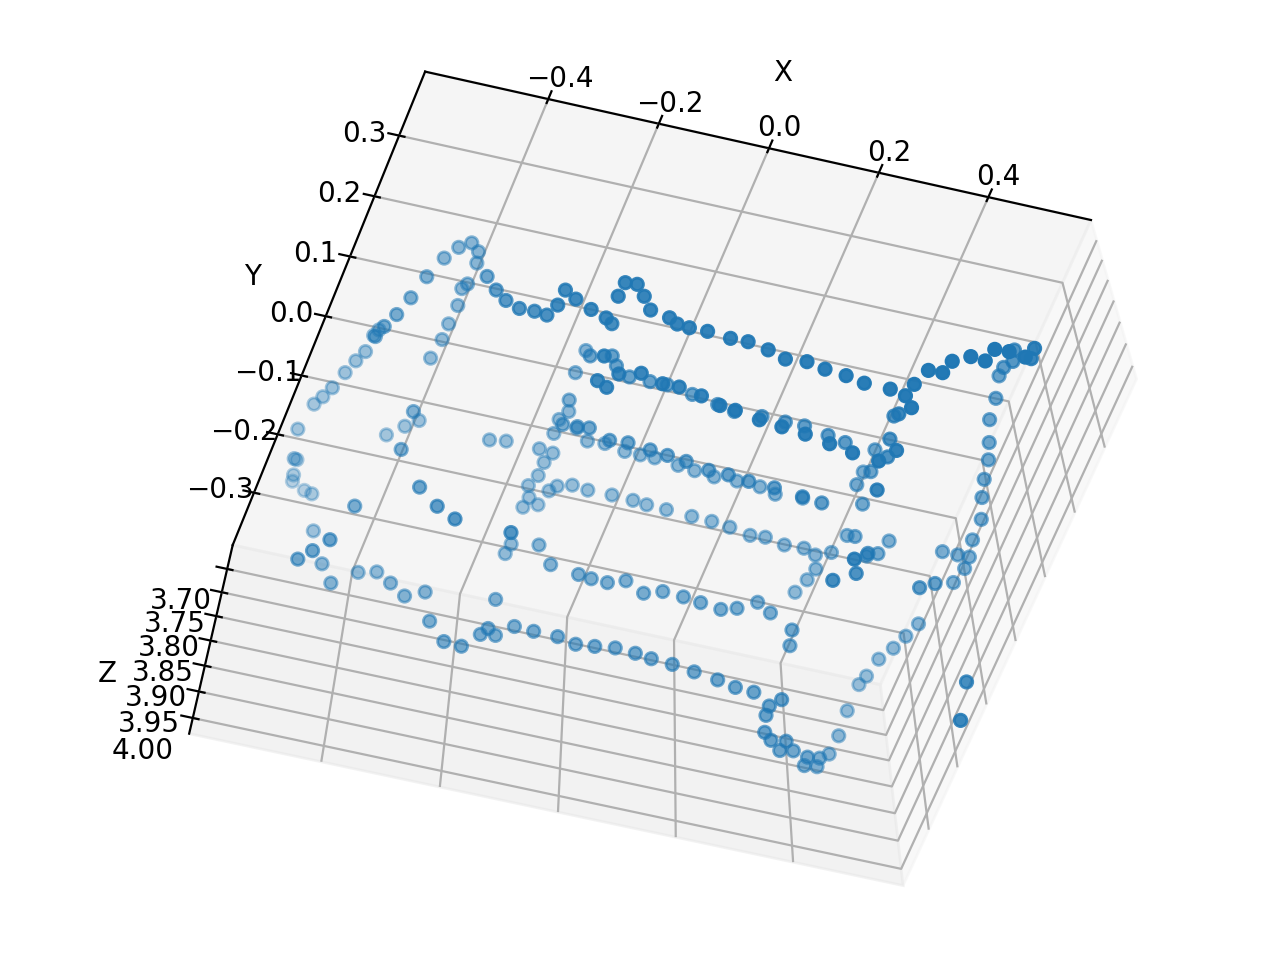
\includegraphics[width=0.4\textwidth]{results/q4_2_2.png}}
\subfigure[]{
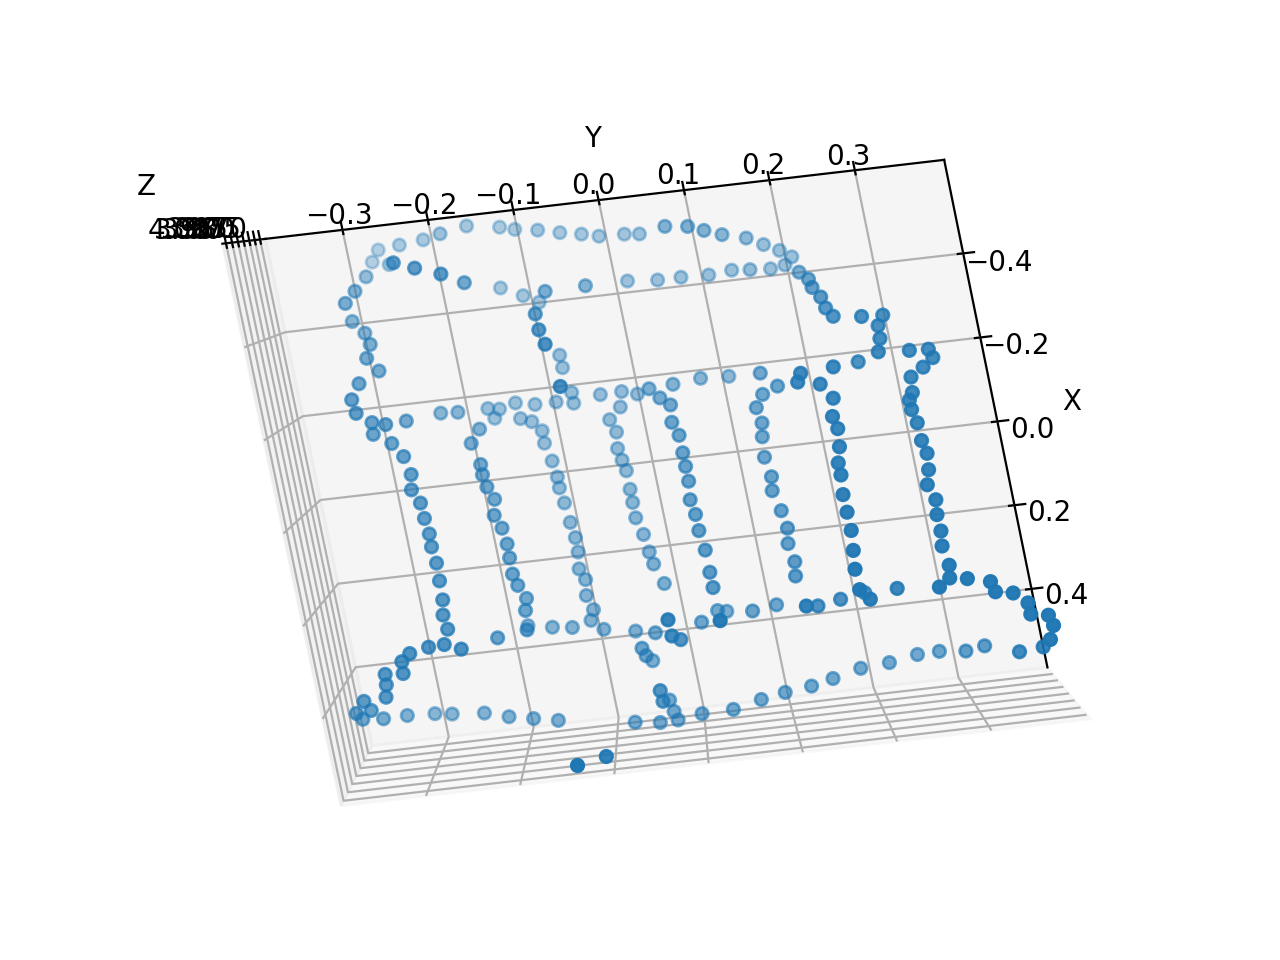
\includegraphics[width=0.4\textwidth]{results/q4_2_3.png}}
\subfigure[]{
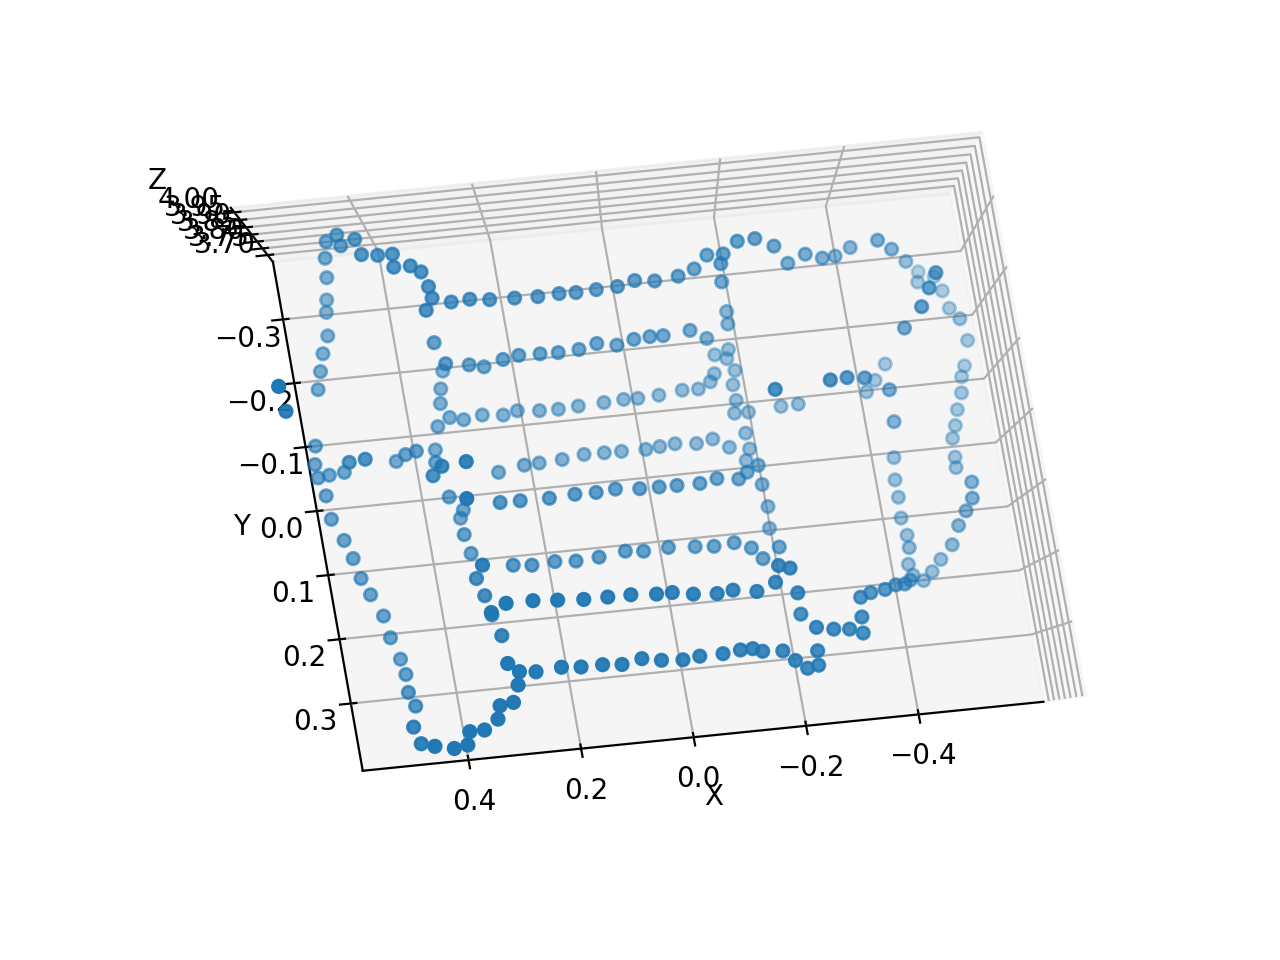
\includegraphics[width=0.4\textwidth]{results/q4_2_4.png}}
\caption{3D Visualization}
\end{figure}

\section{Bundle Adjustment}

\paragraph{Q5.1}~{}

Using the noisy correspondences, without RANSAC, the visualization of epipolar lines is like:
\begin{figure}[H]
\centering
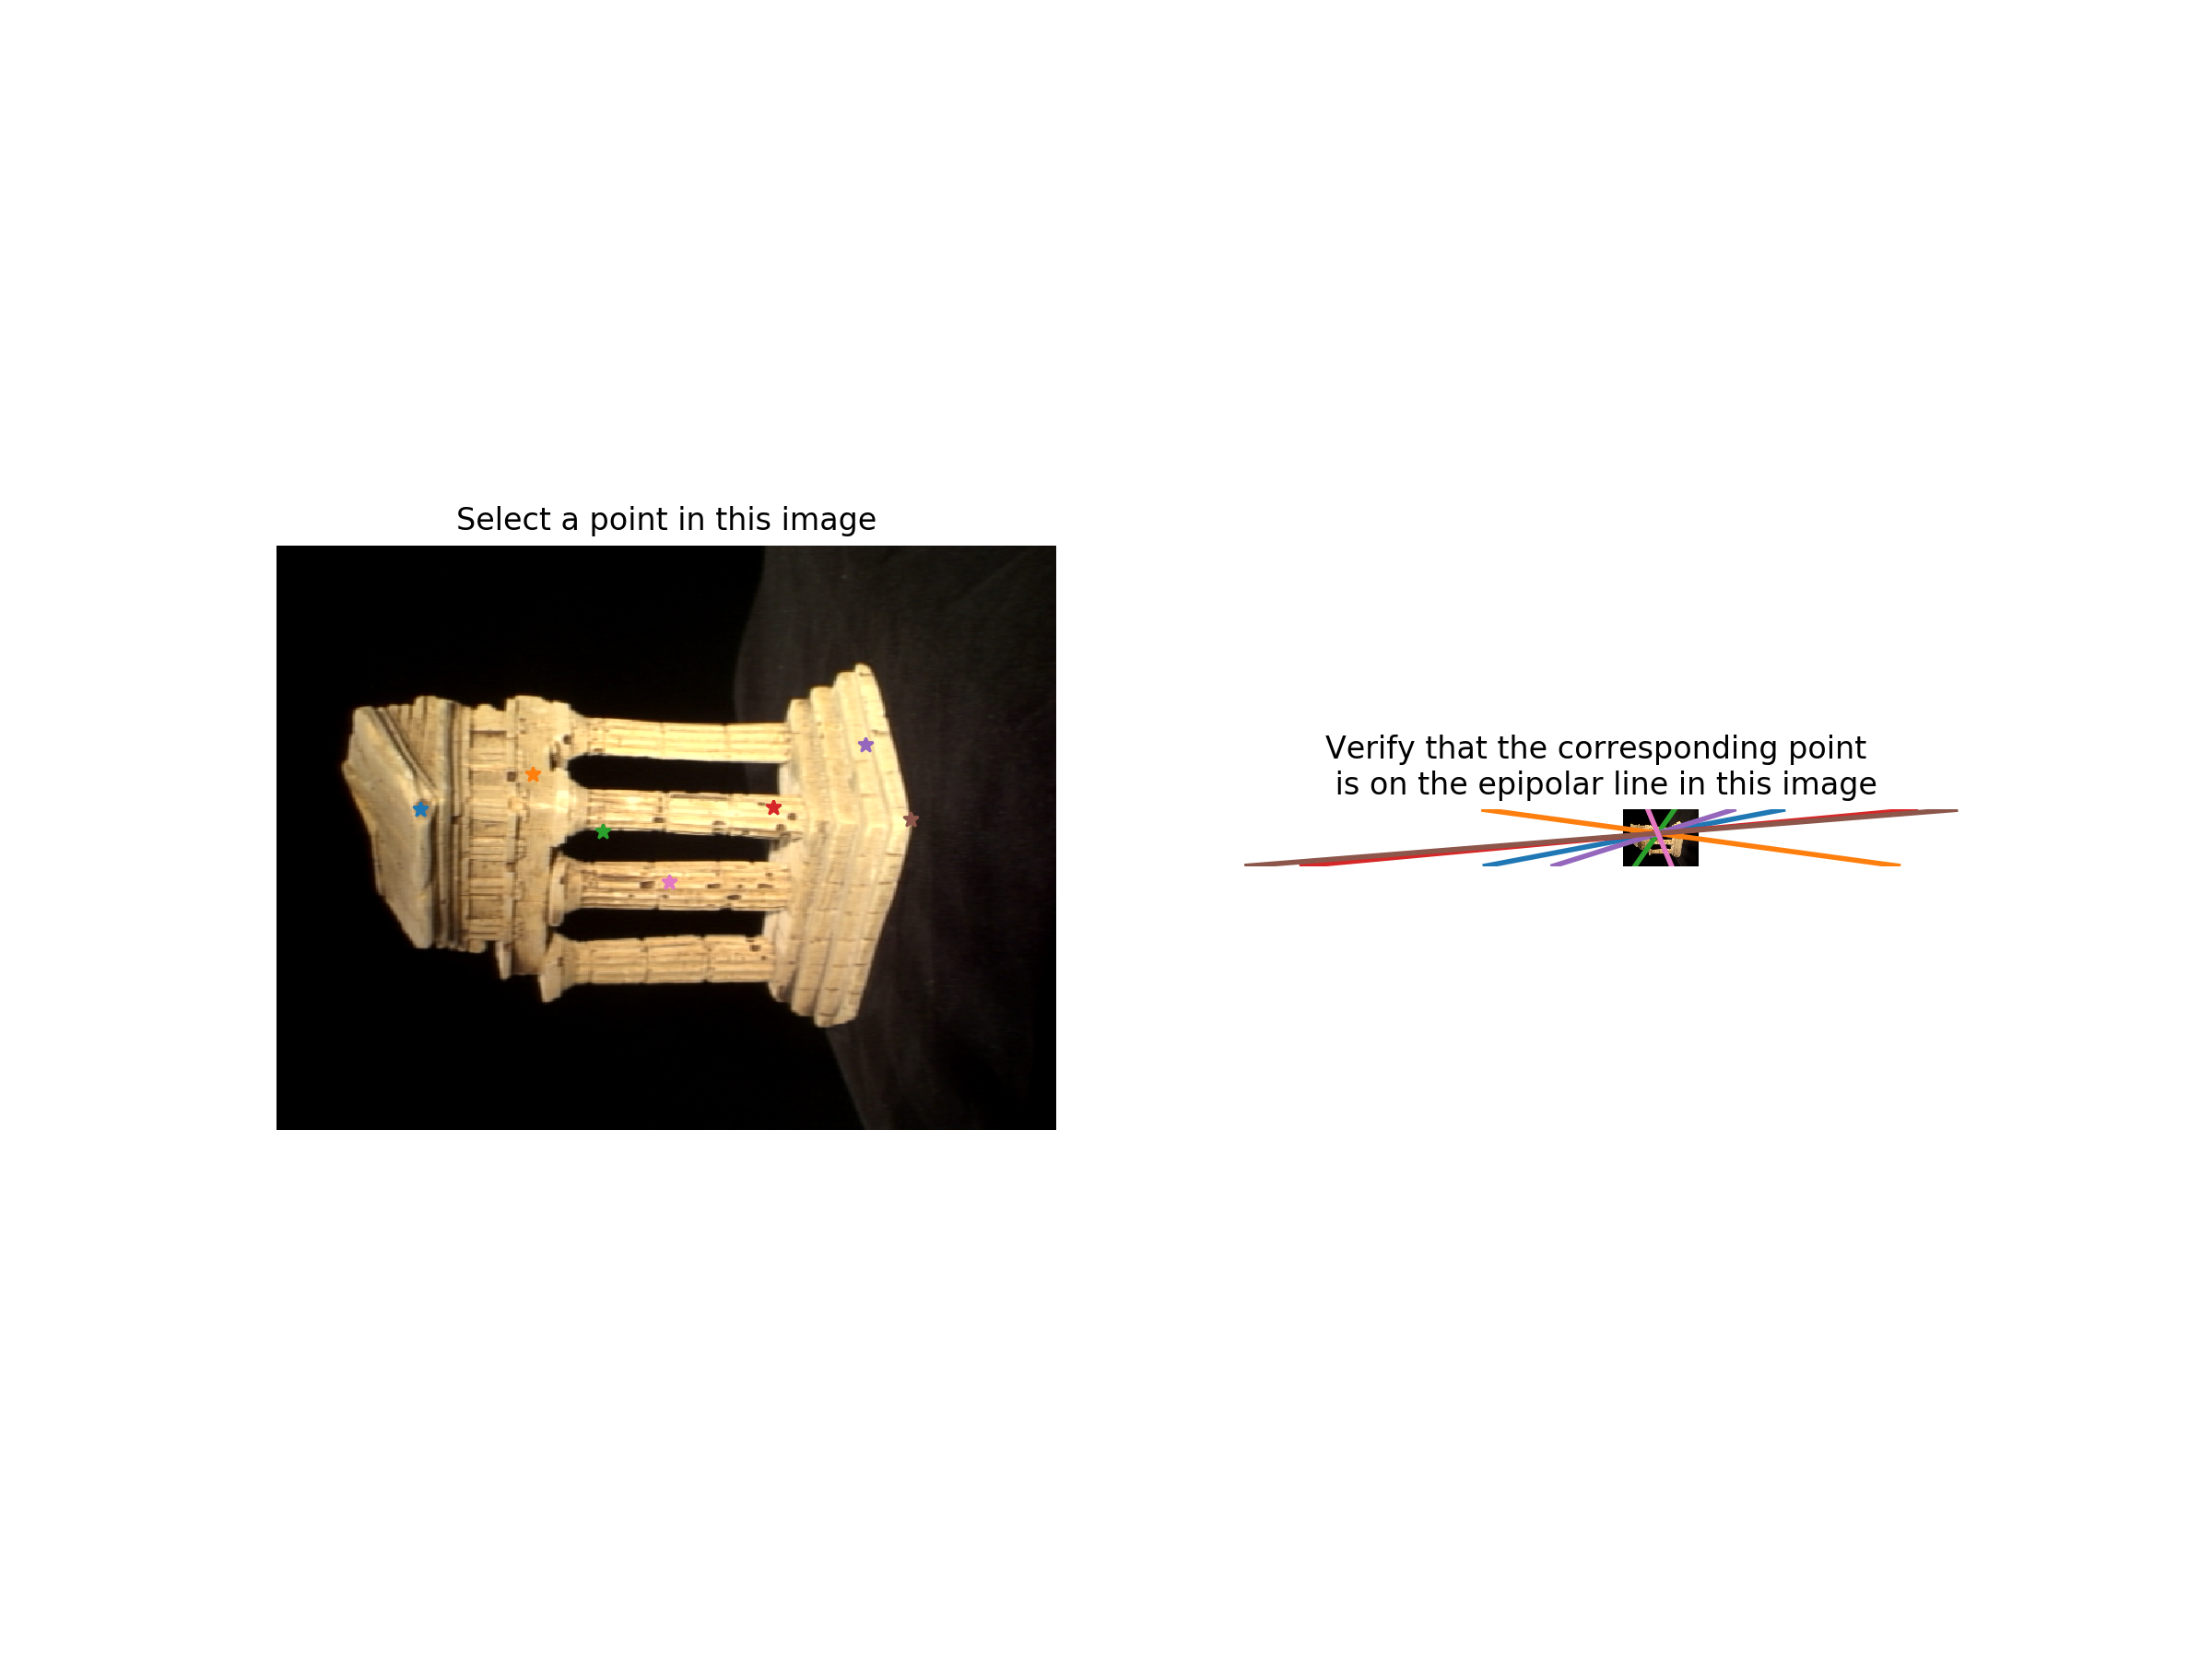
\includegraphics[width=0.6\textwidth]{results/q5_1_without.png}
\caption{Visualization without RANSAC}
\end{figure}

With RANSAC implemented, the result looks much better:
\begin{figure}[H]
\centering
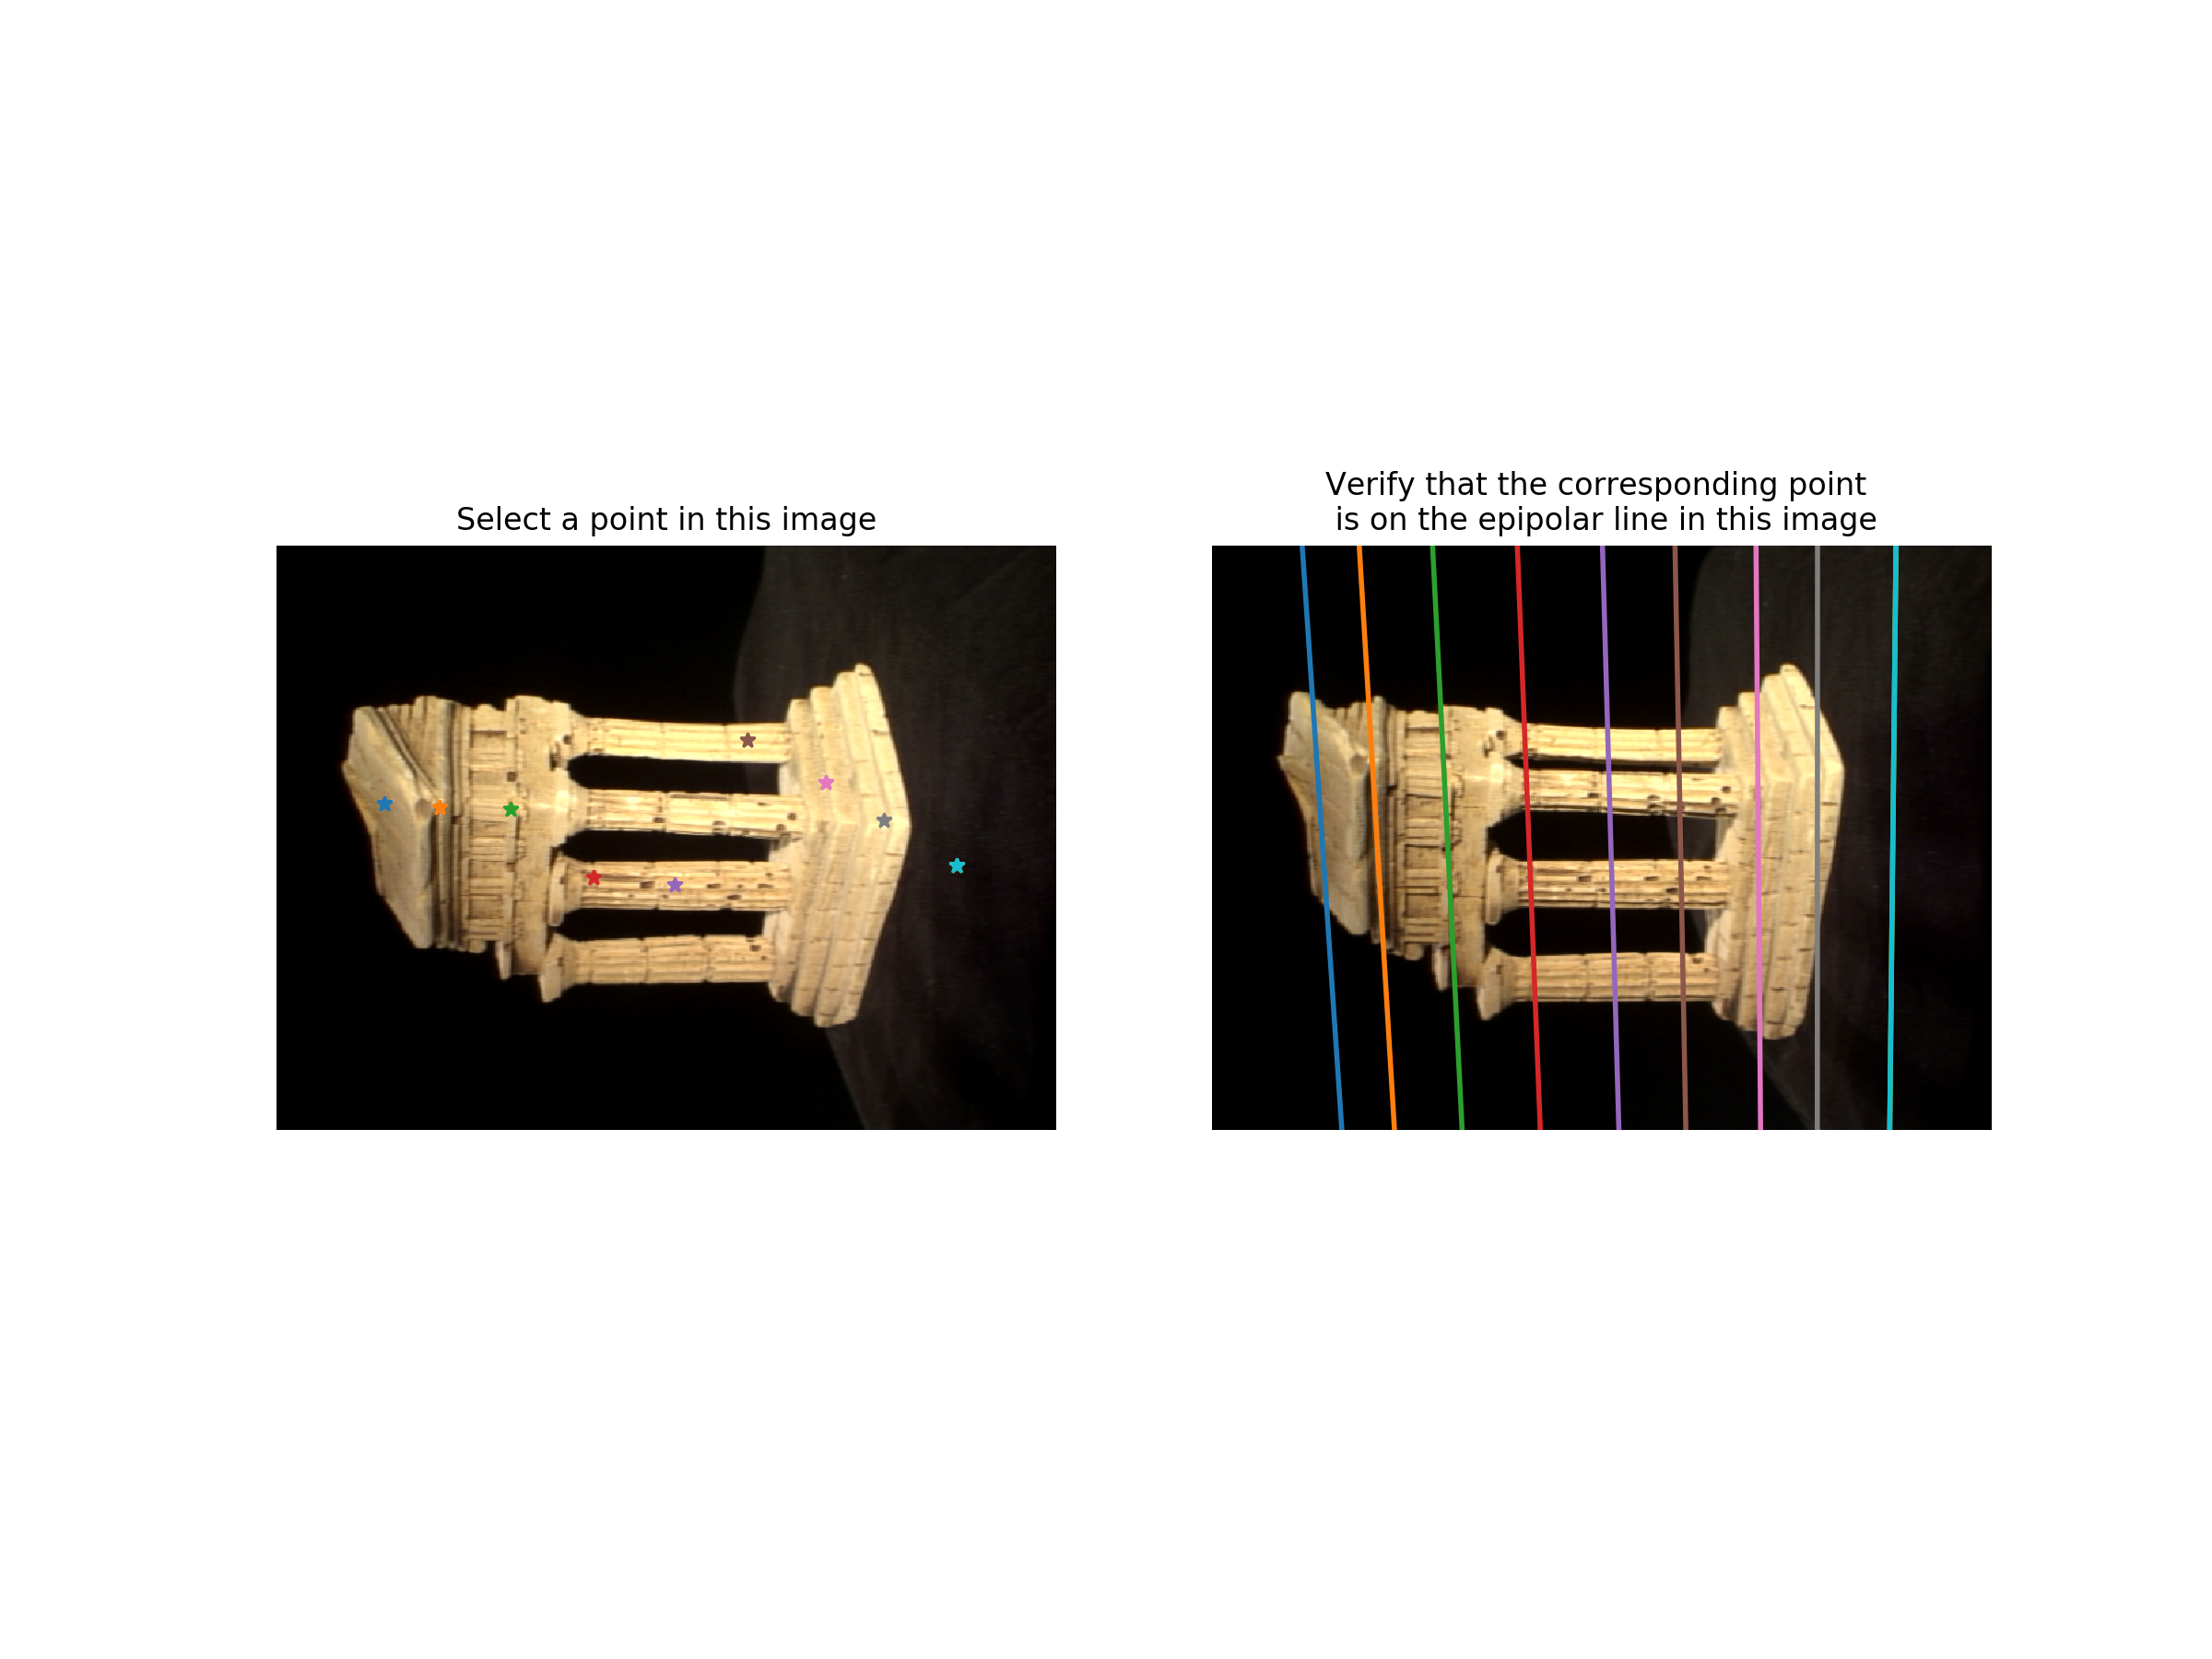
\includegraphics[width=0.6\textwidth]{results/q5_1_with.png}
\caption{Visualization with RANSAC}
\end{figure}

Obtained fundamental matrix $\bold{F}$ is:
\begin{equation}
	\bold{F} = \begin{bmatrix} 1.44845968e-08 & -3.12242026e-07 & 1.07078108e-03 \\
	1.67046292e-07 & 1.00324202e-08 & -8.51505084e-05 \\
	-1.04288634e-03 & 9.23538949e-05 & -2.07767875e-03
	\end{bmatrix}
\end{equation}

For fundamental matrix, we have:
\begin{equation}
	\tilde{\bold{x}_2}^T\bold{F}\tilde{\bold{x}_1} = 0
\end{equation}
So the error metrics used to determine if point $i$ is an inlier is:
\begin{equation}
	err = abs\left(\tilde{\bold{x}_{2i}}^T\bold{F}\tilde{\bold{x}_{1i}}\right)
\end{equation}
Set tolerance as $0.8$ and after $100$ iterations, the $\bold{ransacF}$ function was able to find an ideal enough matrix $\bold{F}$.

While tuning the parameters, turning the tolerance to a smaller number would decrease the inlier number, which would cause lower accuracy for RANSAC, and with more iterations, RANSAC would be able to find a better solution.

\paragraph{Q5.3}~{}

The resulting images are shown below:
\begin{figure}[H]
\centering
\subfigure[without bundle adjustment]{
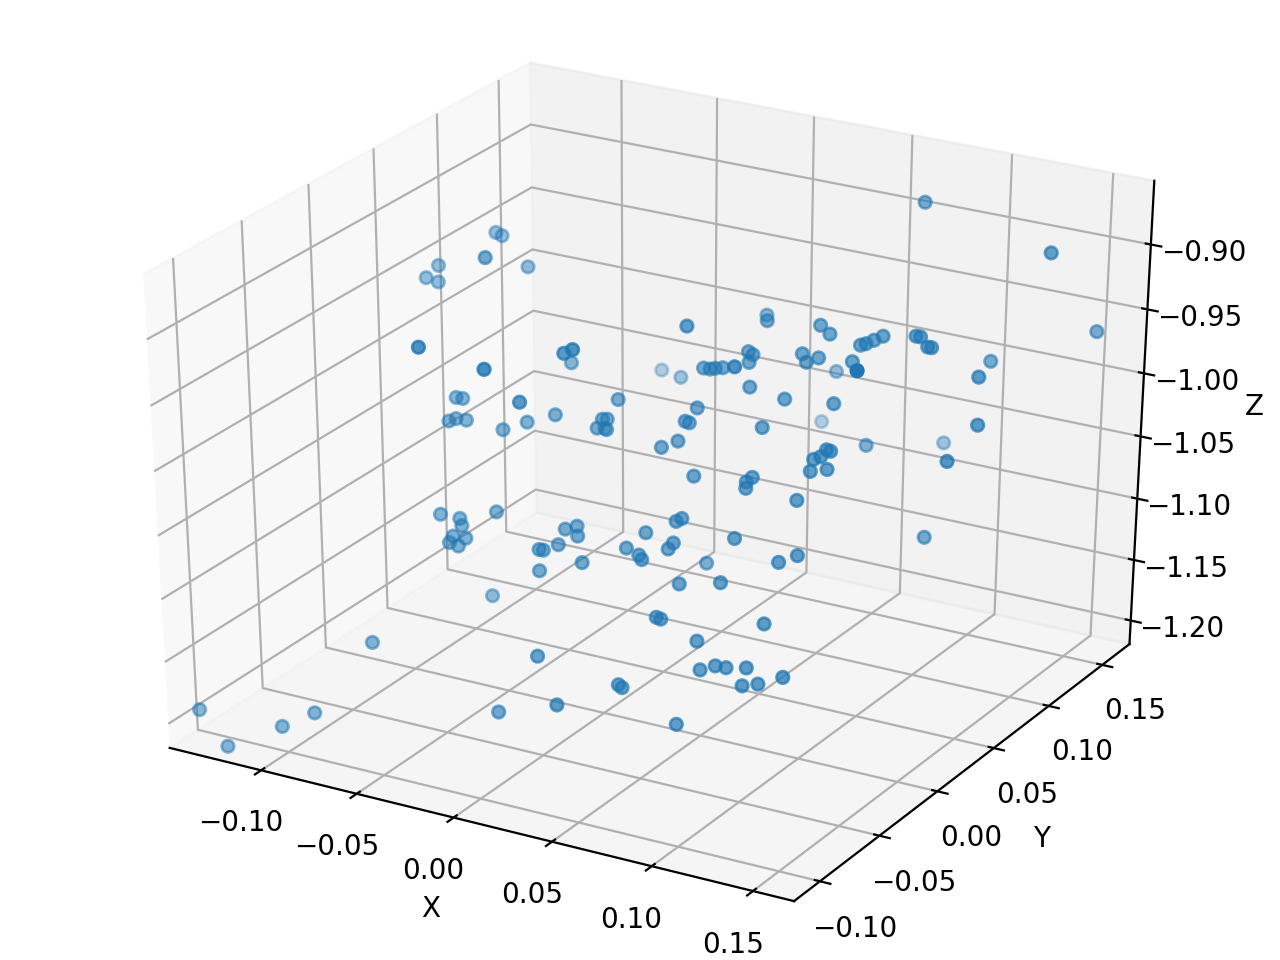
\includegraphics[width=0.5\textwidth]{results/q5_3_without.png}}
\subfigure[with bundle adjustment]{
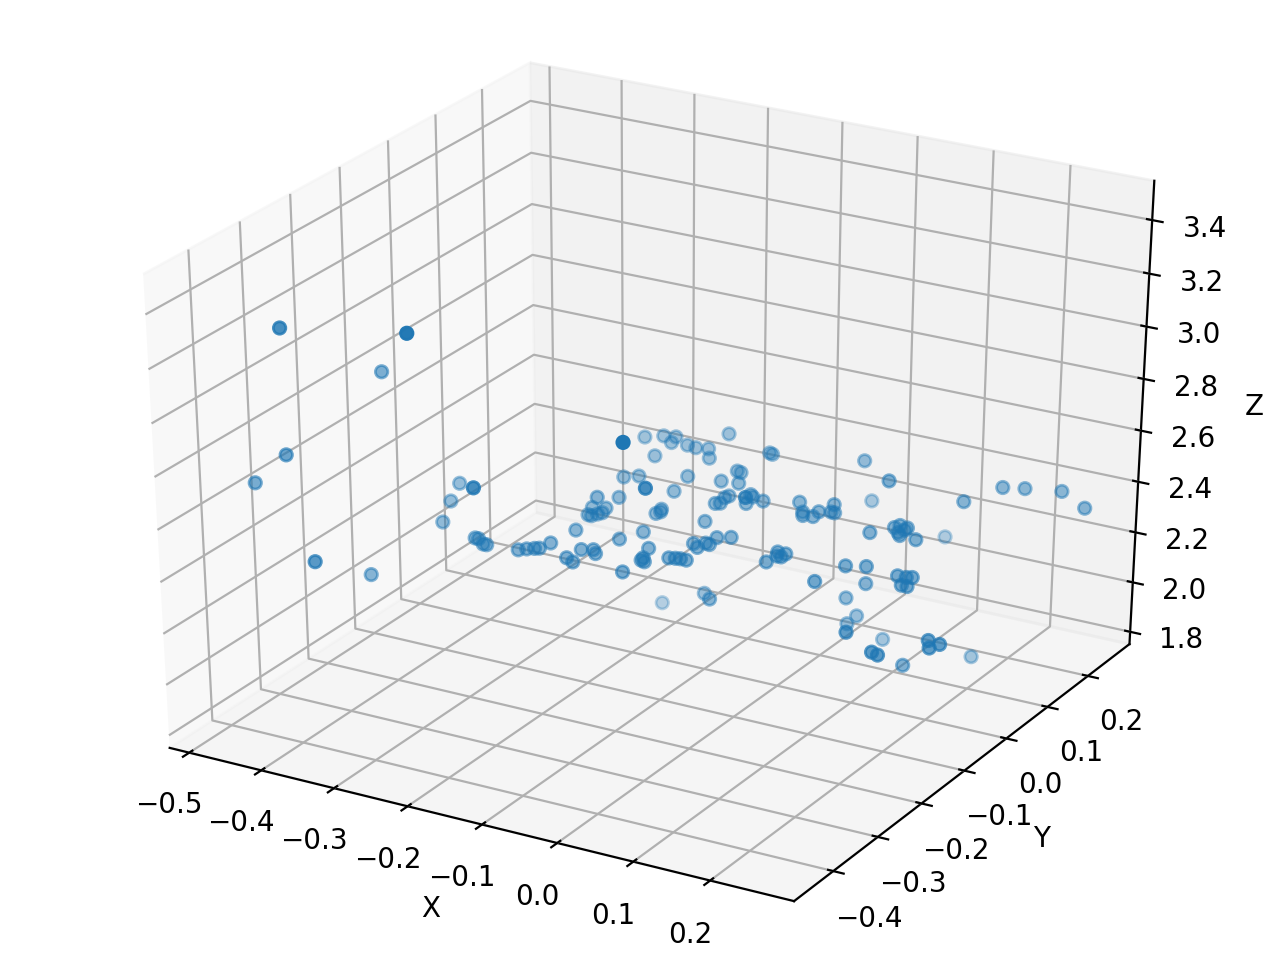
\includegraphics[width=0.5\textwidth]{results/q5_3_with.png}}
\caption{3D Reconstruction with Noisy Data}
\end{figure}

Without bundle adjustment, the reprojection error is $51.484053051875$, while with bundle adjustment the error is $32.15606321697$, which significantly decreased.

\section{Multi View Keypoint Reconstruction}

\paragraph{Q6.1}~{}

In this case, I used the triangulate function I've written before to calculate $3$ sets of $\begin{bmatrix} \bold{w} & err \end{bmatrix}$, and compared the errors to decide the one $\bold{w}$ with the smallest error, the chose this $\bold{w}$ as the one used in reconstruction. An example resulting image is shown below:
\begin{figure}[H]
\centering
\subfigure[]{
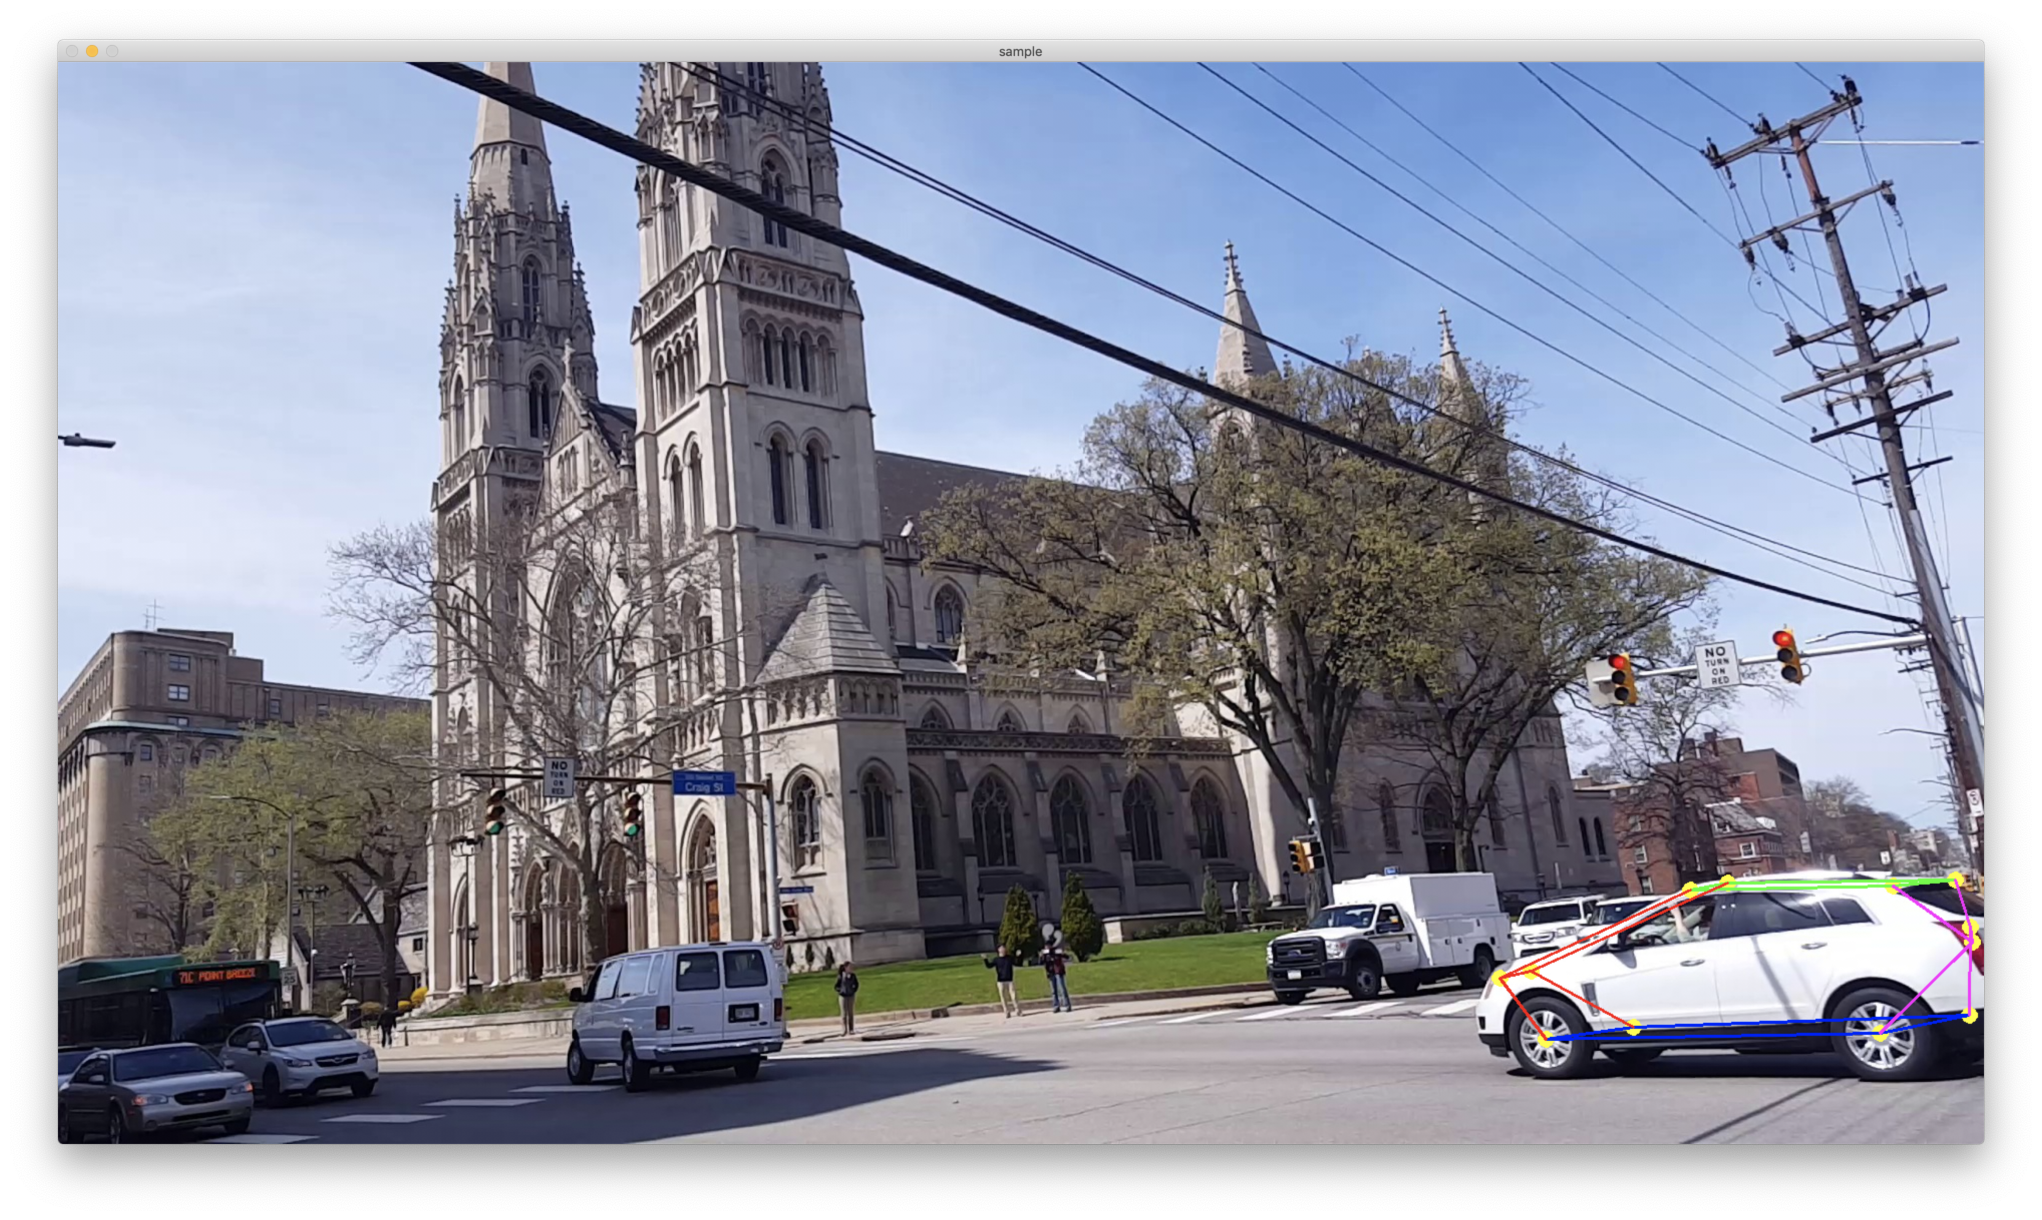
\includegraphics[width=0.3\textwidth]{results/c6_1_1.png}}
\subfigure[]{
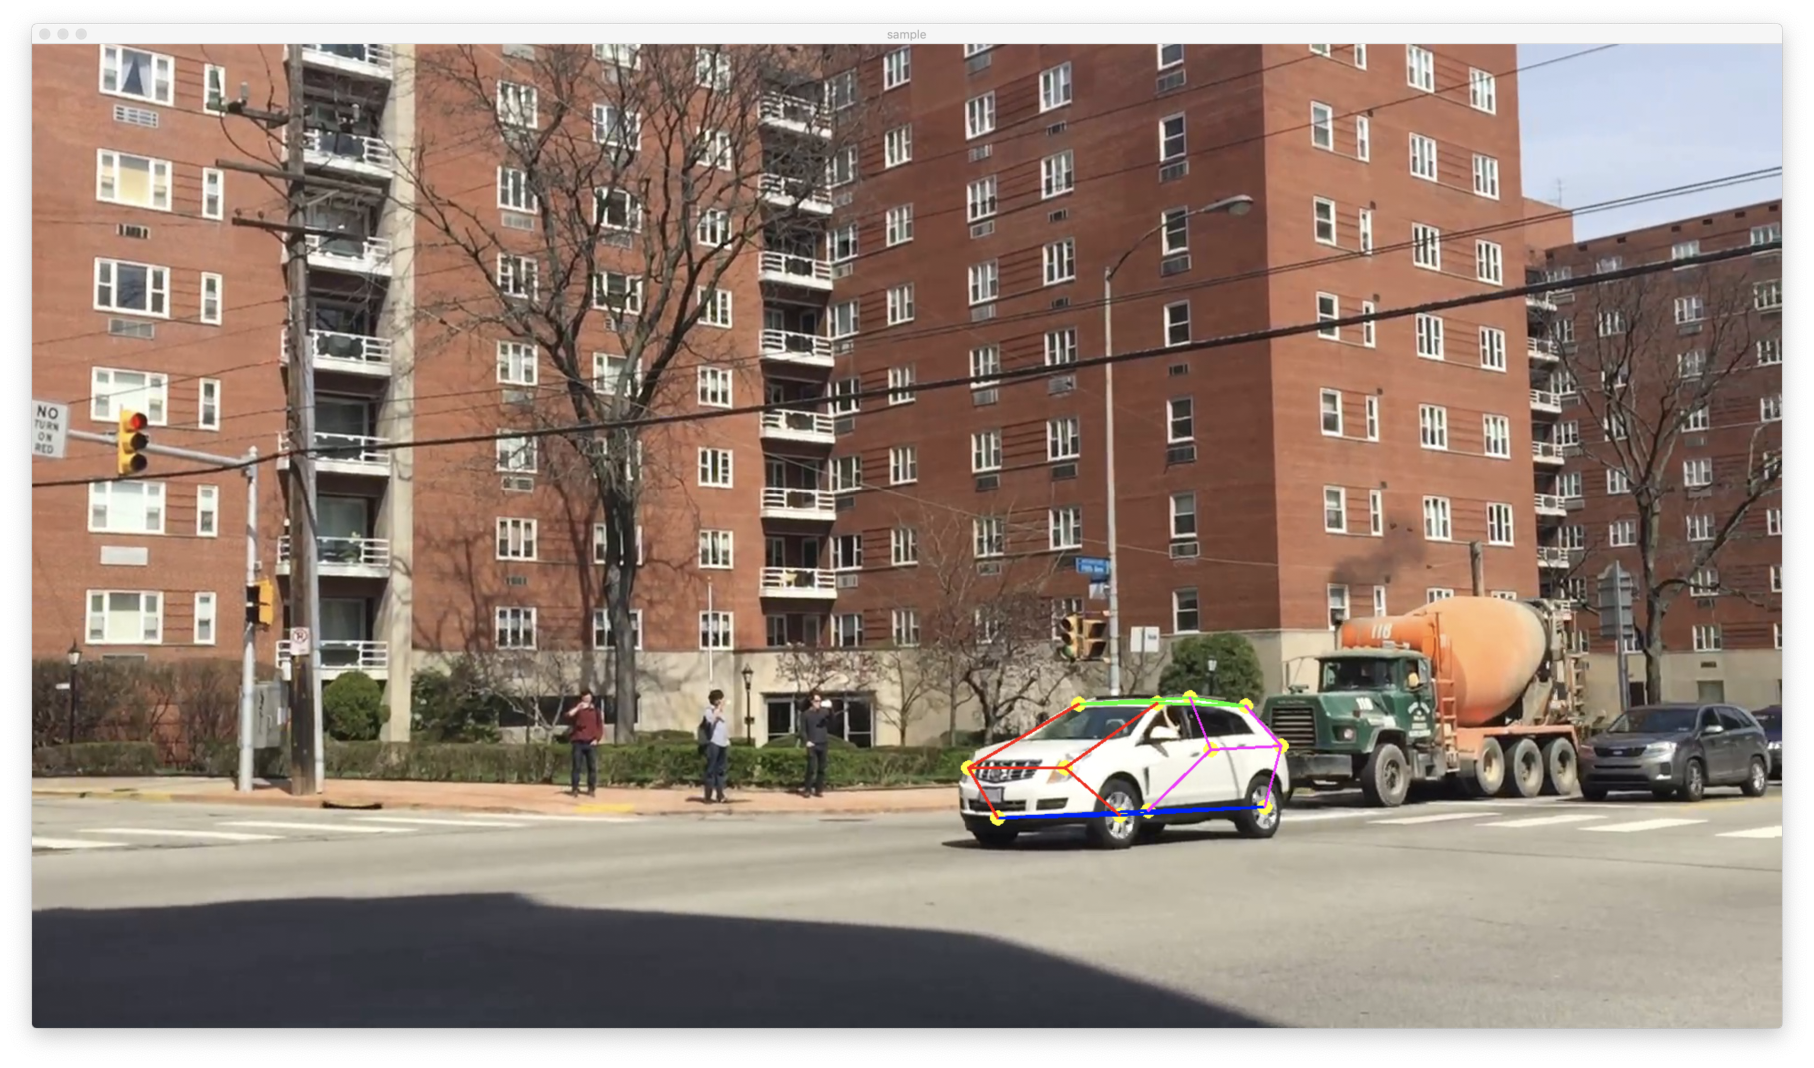
\includegraphics[width=0.3\textwidth]{results/c6_1_2.png}}
\subfigure[]{
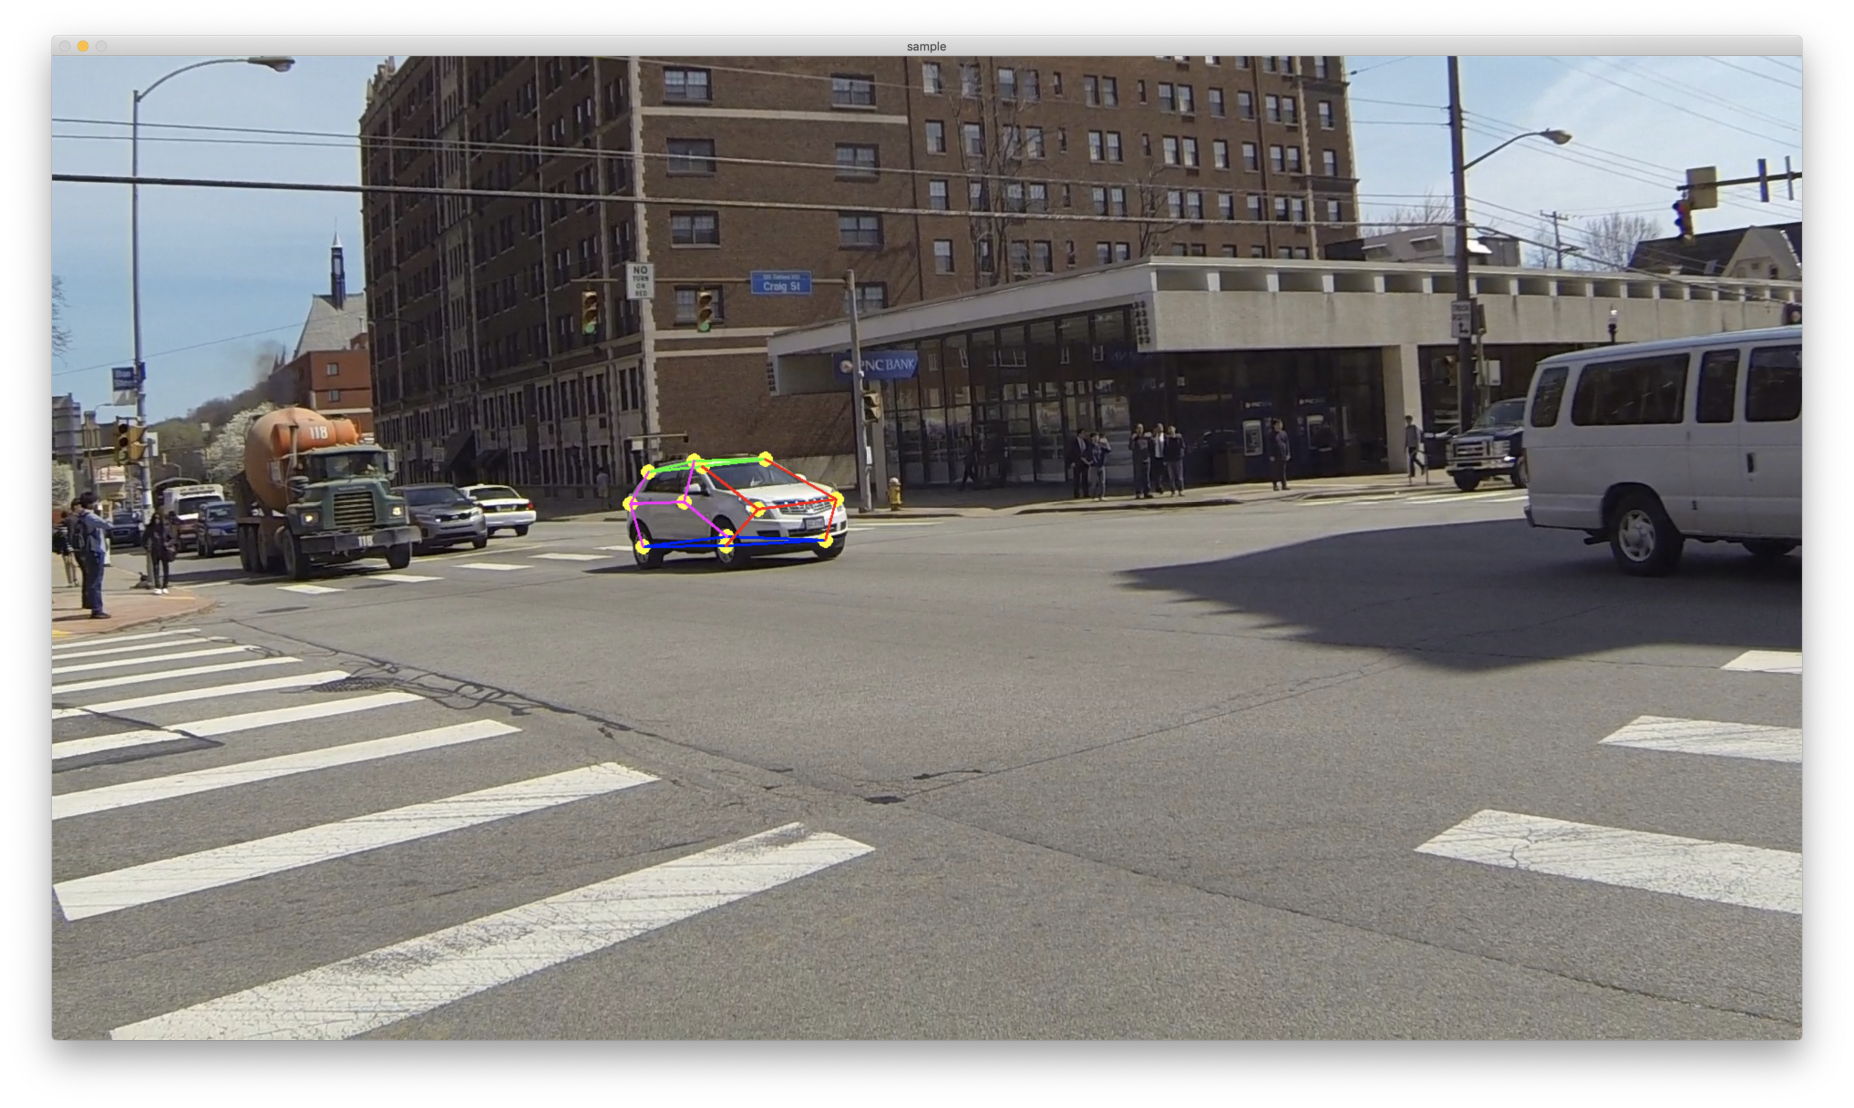
\includegraphics[width=0.3\textwidth]{results/c6_1_3.png}}
\subfigure[]{
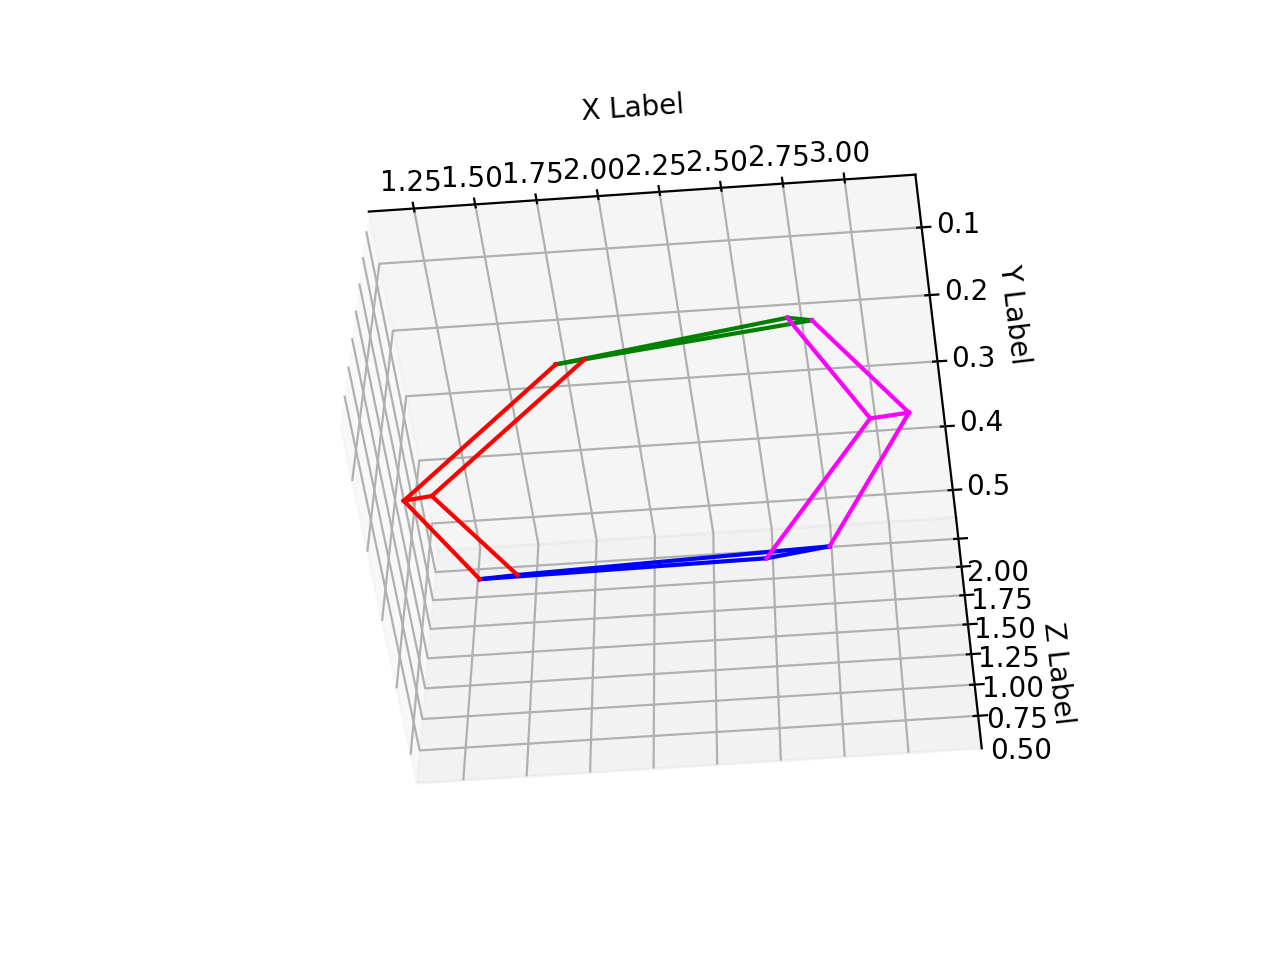
\includegraphics[width=0.3\textwidth]{results/q6_1_1.png}}
\subfigure[]{
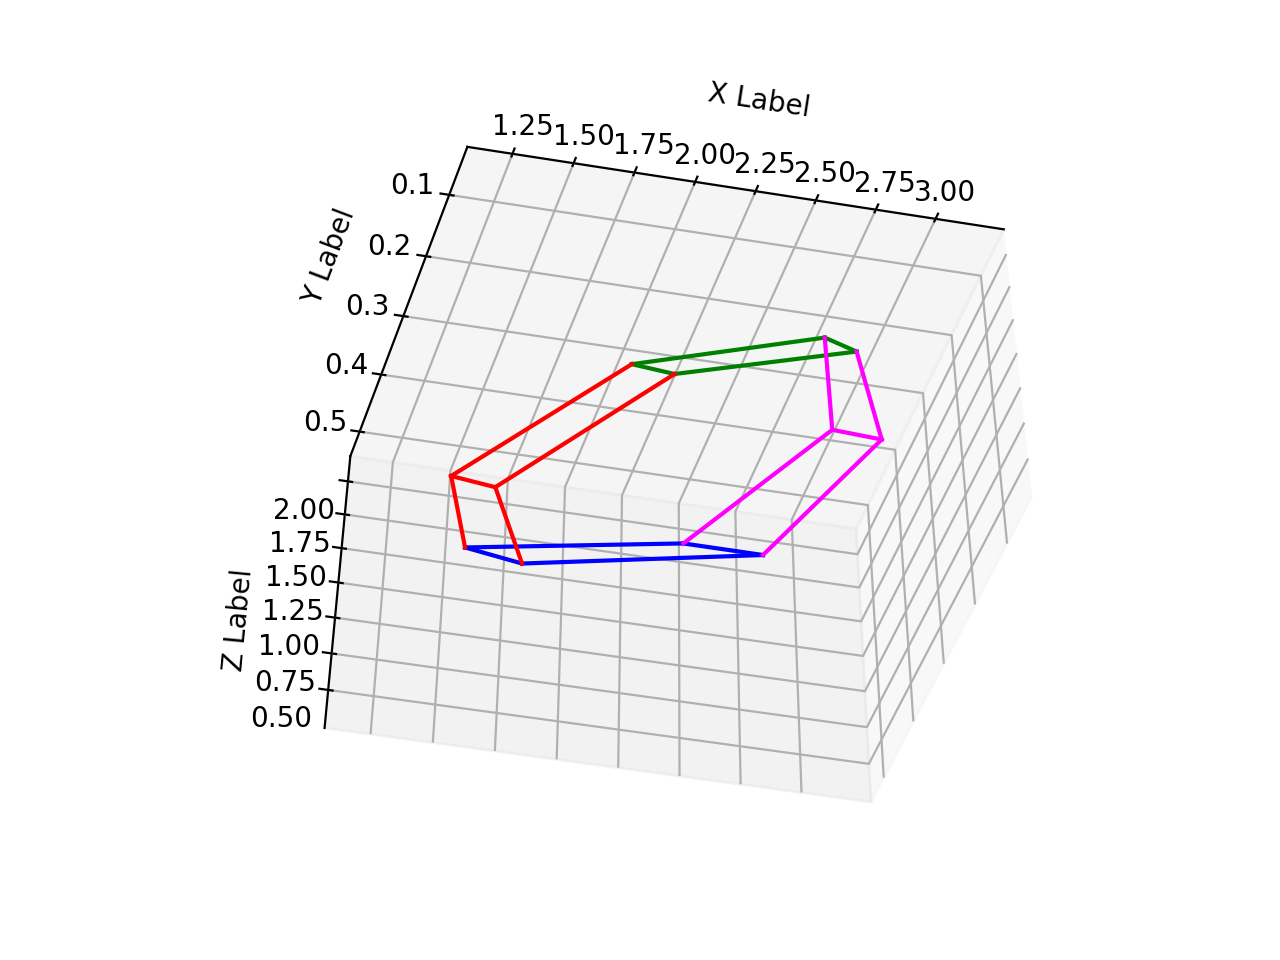
\includegraphics[width=0.3\textwidth]{results/q6_1_2.png}}
\subfigure[]{
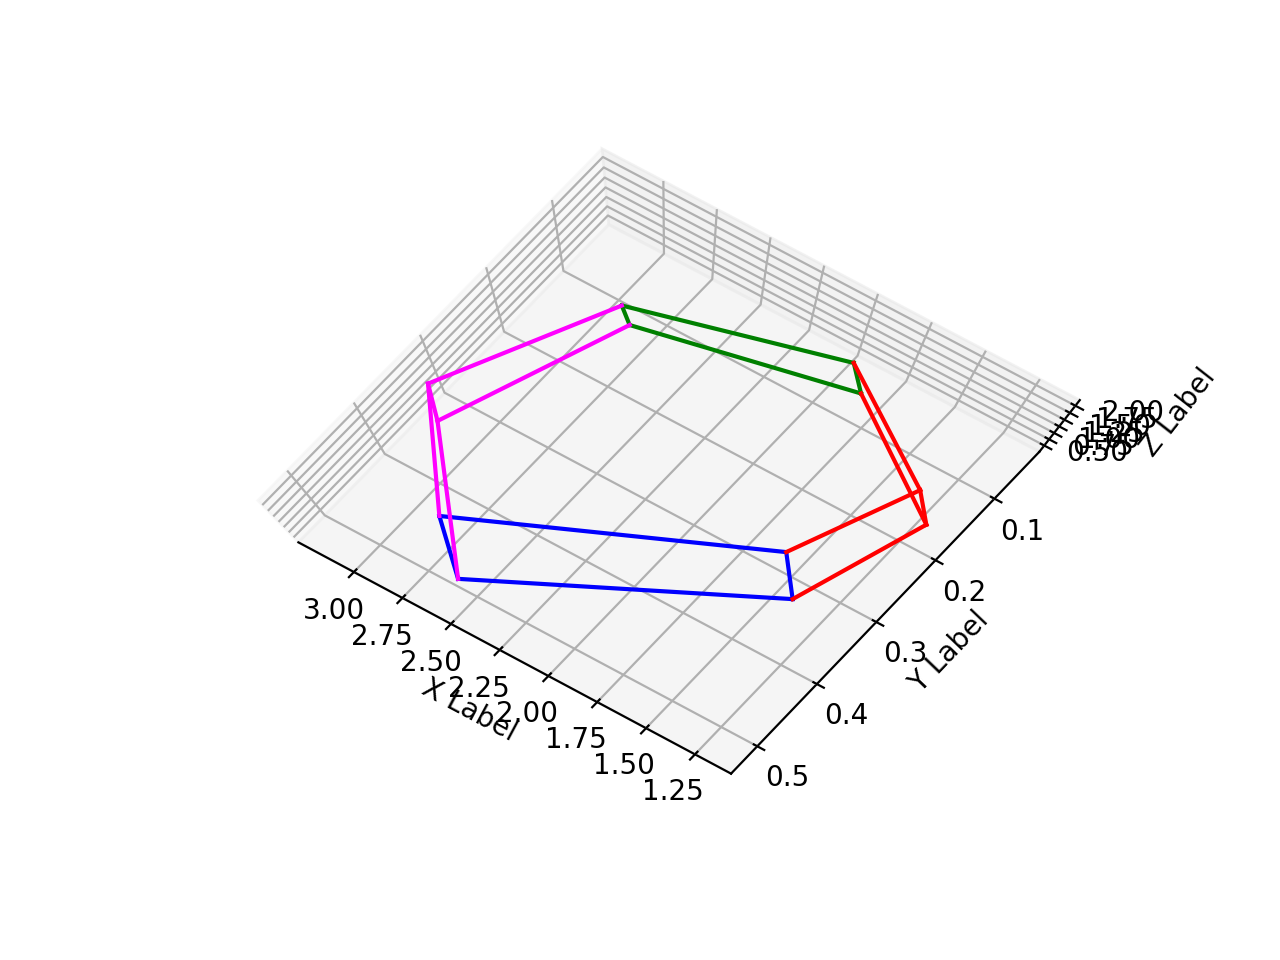
\includegraphics[width=0.3\textwidth]{results/q6_1_3.png}}
\caption{Detections and the Reconstructions from Multiple Views}
\end{figure}

Tuning the parameter threshold would influence the accuracy in keypoints detection, with lower threshold would lead to more accurate detection and reconstruction. The reconstruction error is $724.8793276$.

\paragraph{Q6.2}~{}

The reconstruction result is shown below:
\begin{figure}[H]
\centering
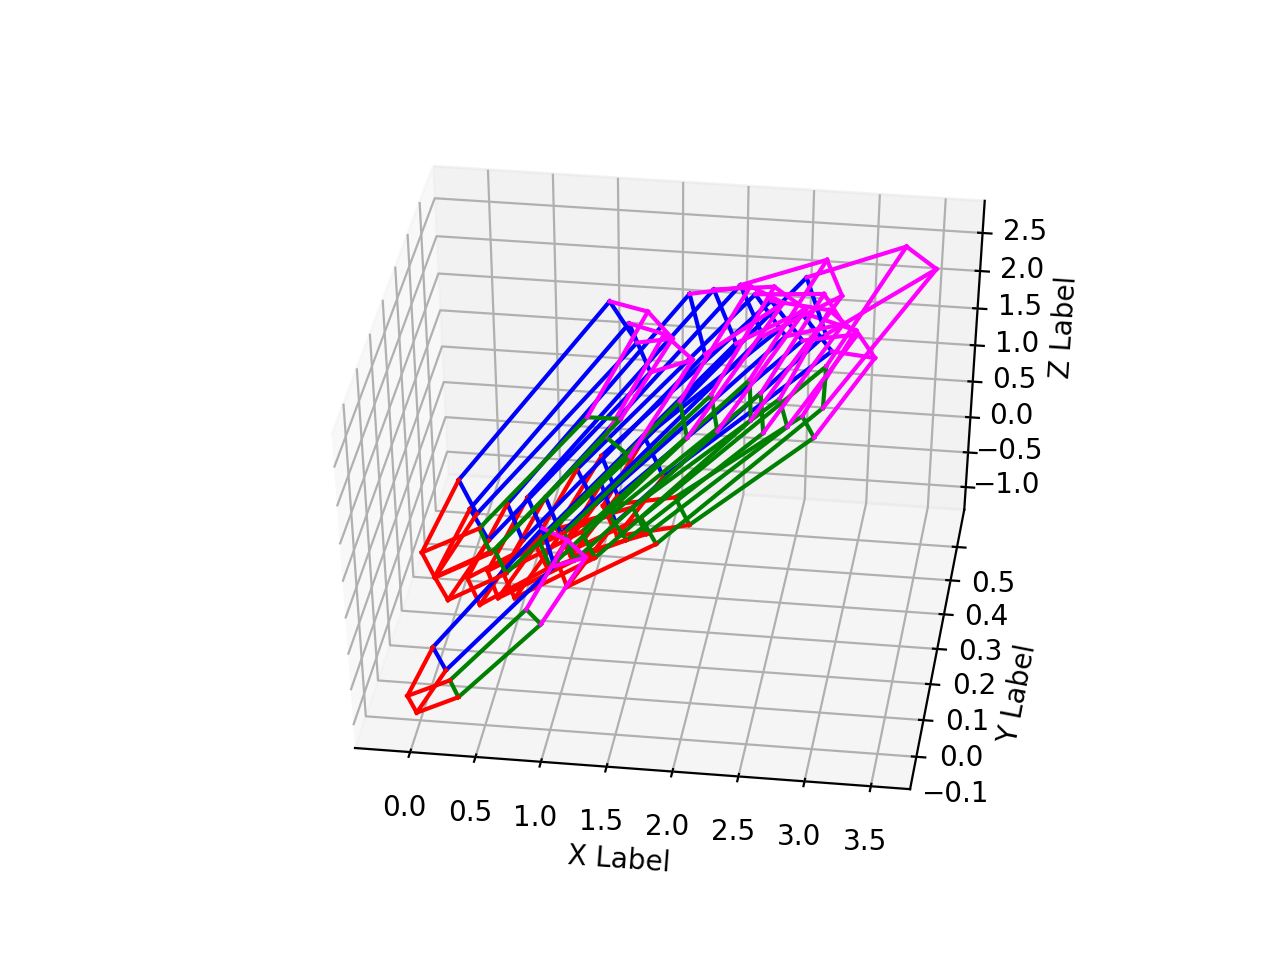
\includegraphics[width=0.8\textwidth]{results/q6_2.png}
\caption{Spatiotemporal Reconstruction}
\end{figure}

\end{document}
